%%%%%%%%%%%%%%%%%%%%%%%%%%%%%%%%%%%%%%%%%%%%%%%%%%%%%%%%%%%%%%%%%%%%%%%%%%%%%%%%
%                                                                              %
%  HIGZ/HPLOT User Guide -- LaTeX Source                                       %
%                                                                              %
%  Chapter: HPLOT reference manual                                             %
%                                                                              %
%  This document needs the following external EPS files:                       %
%           hplset.eps                                                         %
%           btyp.eps                                                           %
%           ndvx.eps                                                           %
%           ndvy.eps                                                           %
%           hplotscat.eps                                                      %
%           hplotbox.eps                                                       %
%           hplotarr.eps                                                       %
%           hplotcont.eps                                                      %
%           hplotcol.eps                                                       %
%           hplottext.eps                                                      %
%           hplotchar.eps                                                      %
%           hplotlego.eps                                                      %
%           hplotlego1.eps                                                     %
%           hplotlego2.eps                                                     %
%           hplotsurf.eps                                                      %
%           hplotsurf1.eps                                                     %
%           hplotsurf2.eps                                                     %
%           hplotsurf3.eps                                                     %
%           hplotsurf4.eps                                                     %
%           hplotlegopol.eps                                                   %
%           hplotlegocyl.eps                                                   %
%           hplotlegosph.eps                                                   %
%           hplotlegopsd.eps                                                   %
%           hplotsurfpol.eps                                                   %
%           hplotsurfcyl.eps                                                   %
%           hplotsurfsph.eps                                                   %
%           hplotsurfpsd.eps                                                   %
%                                                                              %
%  Editor: Michel Goossens / CN-AS                                             %
%  Last Mod.: 14 Sept 1993 mg                                                  %
%                                                                              %
%%%%%%%%%%%%%%%%%%%%%%%%%%%%%%%%%%%%%%%%%%%%%%%%%%%%%%%%%%%%%%%%%%%%%%%%%%%%%%%%
\Filename{H1HPLOTIntroduction}
\chapter{Introduction}

\HPLOT{} is a \FORTRAN{} callable facility for producing \HBOOK\cite{bib-HBOOK}
output on graphic devices other than the line printer. Its main design objective
is to be able to produce drawings and slides of a quality suitable for talks and
publications. To this end, it does not produce all the numeric information of
the \HBOOK{} output routines (which give what can be regarded as working
histograms) but, on the other hand, it is not restricted by the line printer
resolution or character size. The reader is of course supposed to be familiar
with the \HBOOK{} package.

The present version of \HPLOT{} has been developed in the context of the Physics
Analysis Workstation project \PAW\cite{bib-PAW}.

HPLOT can be used either in {\bf BATCH} mode or interactively with PAW. When
running in {\bf BATCH}, one can write a metafile via the \HIGZ{}/\GKS{} packages
and interpret these metafiles using the standard utilities such as
\Pind{GRCONV}, \Pind{GRVIEW} and \Pind{GRPLOT}
(see e.g. \cite{bib-GKS1,bib-GKS2}). \PS{} file can also be produce with the
native \HIGZ{} \PS{} driver. This way is certainly now the most popular because
it doesn't need any translation programs to generate the paper output.

Users are strongly encouraged to use the \PAW{} system to make good quality
pictures. The complete \HPLOT{} functionality described in this manual is
available interactively in \PAW.

\index{batch}
\index{interactive session}
\index{slides}
\index{quality!of pictures}
\index{graphics}
\index{metafile}


\Filename{H2Asimpleexample}
\section{A simple example}
As an introductory example to \HPLOT{} consider an already existing program
using \HBOOK, where one wants to plot all created histograms saving all pictures
into a \GKS{} or \PS{} metafile.
\index{metafile}
\index{IBM!VM/CMS}
\index{VM/CMS!IBM system}
\begin{XMPt}{Simple \HPLOT{} program}
       PROGRAM TEST
       COMMON/PAWC/H(20000)
*
       CALL HLIMIT(20000)         ! Initialize HBOOK
       CALL HBOOK1(...            ! Book and fill histograms with HBOOK
       CALL HBOOK2(...
*
       CALL HISTDO                ! Print all histograms on lineprinter
*
       CALL HPLINT(0)             ! Initialize HPLOT
       CALL HPLCAP(-3)            ! Open metafile on unit 3
       CALL HPLOT(0,' ',' ',0)    ! Write all histograms to metafile
       CALL HPLEND                ! Close HPLOT
       END
\end{XMPt}
On VM/CMS a file definition
\Lit{FILEDEF 3 DISK \HPLOT{} METAFILE A (RECFM F LRECL 80}
must have been made beforehand for the output metafile \Lit{HPLOT METAFILE}.
The latter can be visualized on various devices as desired, e.g. with
the \Pind{GRVIEW} utility if it is a \GKS{} metafile or with any \PS{}
previewer if it is a \PS{} file.


\Filename{H1ReferenceGuide}
\chapter{Reference Guide}


\Filename{H2OverviewofHPLOTcalls}
\section{Overview of \protect\HPLOT{} calls}

{\arraystretch=0.95%
\begin{tabularx}{\textwidth}{@{}l@{\qquad}Xr}
\bf Name      &\bf Action                                 & \bf Page          \\
[2mm]
\Rind{HPLABL} &to define alphanumeric labels lists        &\pageref{HPLABL}   \\
\Rind{HPLAER} &to draw asymetric error bars               &\pageref{HPLAER}   \\
\Rind{HPLARC} &to draw an arc of circle                   &\pageref{HPLARC}   \\
\Rind{HPLAX}  &to add a comment to the axes               &\pageref{HPLAX}    \\
\Rind{HPLBOX} &to draw a box on the picture               &\pageref{HPLBOX}   \\
\Rind{HPLCAP} &to switch or/off metafile output           &\pageref{HPLCAP}   \\
\Rind{HPLCOM} &to add a comment                           &\pageref{HPLCOM}   \\
\Rind{HPLCON} &to draw a contour plot                     &\pageref{HPLCON}   \\
\Rind{HPLDO}  &to plot all histograms (like \Rind{HISTDO})&\pageref{HPLDO}    \\
\Rind{HPLEGO} &to plot a scatter plot as a 3 dim view     &\pageref{HPLEGO}   \\
\Rind{HPLEND} &to terminate \HPLOT{}                      &\pageref{HPLEND}   \\
\Rind{HPLERR} &to draw error bars                         &\pageref{HPLERR}   \\
\Rind{HPLFRA} &to define (and draw) a frame               &\pageref{HPLFRA}   \\
\Rind{HPLFUN} &to draw a function                         &\pageref{HPLFUN}   \\
\Rind{HPLGIV} &to return size of the current zone         &\pageref{HPLGIV}   \\
\Rind{HPLINE} &to draw straight lines                     &\pageref{HPLINE}   \\
\Rind{HPLINT} &to initialize \HPLOT{}                     &\pageref{HPLINT}   \\
\Rind{HPLKEY} &to draw a symbol and its explanation       &\pageref{HPLKEY}   \\
\Rind{HPLNT}  &to plot a N-tuple                          &\pageref{HPLNT}    \\
\Rind{HPLNUL} &to draw a picture or zone frame            &\pageref{HPLNUL}   \\
\Rind{HPLNXT} &user routine called before each new frame  &\pageref{HPLNXT}   \\
\Rind{HPLOC}  &for graphics input                         &\pageref{HPLOC}    \\
\Rind{HPLOPT} &to define options                          &\pageref{HPLOPT}   \\
\Rind{HPLOT}  &to plot histograms or plots                &\pageref{HPLOT}    \\
\Rind{HPLPRO} &to plot a scatter plot and its projections &\pageref{HPLPRO}   \\
\Rind{HPLPTO} &wait after each plot                       &\pageref{HPLPTO}   \\
\Rind{HPLSET} &to redefine parameters                     &\pageref{HPLSET}   \\
\Rind{HPLSIZ} &to set or read picture dimensions          &\pageref{HPLSIZ}   \\
\Rind{HPLSOF} &to draw software characters                &\pageref{HPLSOF}   \\
\Rind{HPLSUR} &to plot a scatter plot as a 3 dim view     &\pageref{HPLSUR}   \\
\Rind{HPLSYM} &to draw symbols on the picture             &\pageref{HPLSYM}   \\
\Rind{HPLTAB} &to draw an histogram as a table            &\pageref{HPLTAB}   \\
\Rind{HPLTIT} &to draw a title                            &\pageref{HPLTIT}   \\
\Rind{HPLUSR} &user routine called after each plot        &\pageref{HPLUSR}   \\
\Rind{HPLWIR} &to draw cross-wires on a picture.          &\pageref{HPLWIR}   \\
\Rind{HPLZOM} &to zoom a picture                          &\pageref{HPLZOM}   \\
\Rind{HPLZON} &to split the picture into zones            &\pageref{HPLZON}   \\
\end{tabularx}
}% End of arraystretch


\newpage
\Shubr{HPLABL}{(NUM, NB, CHLAB)}
\Action
By default, labels used by axis are numeric labels. This routine, allows the 
user to define up to nine alphanumeric set of labels (numbered from \Lit{1} to
\Lit{9}). These labels can then be used in subsequent calls producing axis.
This routine limits the lenght of the alphanumeric labels at 32 characters.
\Pdesc
\begin{DLtt}{12345678}
\item[NUM]       List number.
\item[NB]        Number of labels .
\item[CHLAB(NB)] Array of \CHARACTER{} defining the list contents.
\end{DLtt}
See also \Rind{HPLSET}.


\Shubr{HPLAER}{(XU ,YU, DXU1, DXU2, DYU1, DYU2, N, CHOPT, ISYM, USIZE)}
\Action
Allows the user to draw his own (asymetric) error bars on the picture. Error
bars computed by \HBOOK{} are automatically plotted by \HPLOT. They can,
however, be turned off via the routine \Rind{HPLOPT} with the option
'\Oind{NEAH}' (``No Errors And Histogram''). The character with code \Lit{ISYM}
is plotted at the point given by the coordinates \Lit{(XU,YU)}
\Pdesc
\begin{DLtt}{1234567890}
\item[XU]        Array of floating point numbers specifying the X-coordinate of
                 the centre point of the error bars to be drawn.
\item[YU]        Array of floating point numbers specifying the Y-coordinate of
                 the centre point of the error bars to be drawn.
\item[DXU1-DXU2] Arrays of floating point numbers specifying the half length
                 in the X direction of the error bars, i.e. the error bar is
                 drawn from \Lit{XU(I) - DXU1(I)} to \Lit{XU(I) + DXU2(I)}.
\item[DYU1-DYU2] Arrays of floating point numbers specifying the half length
                 in the Y direction of the error bars, i.e. the error bar is
                 drawn from \Lit{YU(I) - DYU1(I)} to \Lit{YU(I) + DYU2(I)}.
\item[N]         Length of the arrays \Lit{XU, YU, DXU1, DXU2, DYU1, DYU2}.
\item[CHOPT]     \CHARACTER{} variable determining the coordinate system of the
                 \Lit{XU...} coordinates:
\begin{DLtt}{12}
  \item[' '] means that the coordinates are expressed in histogram coordinates
             (of the last drawn histogram). Error bars are drawn.
  \item['C'] (or \Lit{'CM'} for compatibility) means that the coordinates are
             expressed in cm.
  \item['W'] a new window is defined and axis are drawn.
  \item['0'] error bars are drawn (default).
  \item['1'] small lines at the end of the error bars are drawn.
  \item['2'] error rectangles are drawn.
  \item['3'] a filled area is drawn through the end points of the vertical 
             error bars.
  \item['4'] a smoothed filled area is drawn through the end points of the 
             vertical error bars.
\end{DLtt}
\item[ISYM]  Code of the symbol to be drawn at each point (see \Rind{HPLSYM}).
             {\tt0} means that no symbols is printed.
\item[USIZE] Size of the symbol to be drawn at each point (see \Rind{HPLSYM}).
             {\tt0} means that no symbols is printed.
\end{DLtt}
\Remarks
\begin{UL}
\item See also \Rind{HPLERR}.
\item The options \Lit{'0'}, \Lit{'1'}, \Lit{'2'}, \Lit{'3'} and \Lit{'4'} can
      be cumulated.
\item \Rind{HPLAER} must be called after \Rind{HPLFRA} or \Rind{HPLOT}.
\end{UL}


\Shubr{HPLARC}{(XC, YC, RAD, PHI1, PHI2)}
\Action
Draws an arc of circle.
\Pdesc
\begin{DLtt}{1234567}
\item[XC]   X coordinate of the centre of the arc in cm.
\item[YC]   Y coordinate of the centre of the arc in cm.
\item[RAD]  Radius of the arc in cm.
\item[PHI1] The arc of circle is drawn from \Lit{PHI1} to \Lit{PHI2} (degrees).
\item[PHI2] If \Lit{PHI1 = PHI2} (0 for instance) then a complete circle is
            drawn.
\end{DLtt}
Note that the line type can be changed with parameter
\Sind{DMOD}in \Rind{HPLSET}.
\Remark
\Rind{HPLARC} is only kept for compatibility with earlier versions. Users are
encouraged to switch to the more powerful \HIGZ{} routine \Rind{IGARC}.


\Shubr{HPLAX}{(CHXTIT, CHYTIT)}
\Action
Prints titles along the X and/or Y axes of the plot.
\Pdesc
\begin{DLtt}{1234567}
\item[CHXTIT] Character string to be printed on the X axis.\\
              {\tt' '} means that no label has to be drawn on the X axis.
\item[CHYTIT] Character string to be printed on the Y axis.\\
              {\tt' '} means that no label has to be drawn on the Y axis.
\end{DLtt}
\Remarks
\begin{UL}
\item Each title is printed either to the right and below the axis (X) or at
      the top and to the left (Y).
\item The position of the axis labels may be redefined with \Rind{HPLSET}
      (\Sind{XLAB} and \Sind{YLAB}).
\item The labels are only printed on an already existing picture, i.e.
      \Rind{HPLAX} must be called {\bf after} \Rind{HPLOT}.
\end{UL}


\Shubr{HPLBOX}{(XLOW, YLOW, XUP, YUP, CHOPT)}
\Action
Draws a rectangular box on the picture. The area delimited by the rectangle is
filled according to the fill area interior style index and fill area style index
set in \Rind{HPLSET} with parameter \Sind{BTYP}, and to the fill area colour
index set in \Rind{HPLSET} with parameter \Sind{BCOL}. The contour is always
drawn.
\Pdesc
\begin{DLtt}{12345}
\item[XLOW]  X coordinate of the lower left hand corner of the box.
\item[YLOW]  Y coordinate of the lower left hand corner of the box.
\item[XUP]   X coordinate of the upper right hand corner of the box.
\item[YUP]   Y coordinate of the upper right hand corner of the box.
\item[CHOPT] Character variable determining the coordinate system of the
             \Lit{XLOW...} coordinates:
\begin{DLtt}{123}
  \item[' '] means that the coordinates are expressed in histogram
             coordinates (of the last drawn histogram).
  \item['C'] (or \Lit{'CM'} for compatibility) means that the coordinates are
             expressed in centimeters.
\end{DLtt}
\end{DLtt}
\Remark
\Rind{HPLBOX} must be called after \Rind{HPLFRA} or \Rind{HPLOT}.


\Shubr{HPLCAP}{(IFILE)}
\Action
Changes the status of metafile and terminal output.
\Pdesc
\begin{DLtt}{12345}
\item[IFILE] Logical unit for the GKS metafile.
\begin{DLtt}{123}
   \item[\phantom{0}10] Enable terminal output and metafile output to \FORTRAN{}
                        unit \Lit{IFILE}
   \item[\phantom{00}0] Enable terminal output only
   \item[-10]           Enable metafile output to \FORTRAN{} unit \Lit{IFILE}
                        only.
\end{DLtt}
\end{DLtt}
\Remark
\Rind{HPLCAP} is only kept for compatibility with previous versions. It is now
strongly recommended to use \HIGZ{} Routine \Rind{IGMETA}
\Lit{(IFILE, METAFILE-TYPE)}, with metafile types \Lit{4}, \Lit{-111}, \Lit{-112},
etc.

\Rind{HPLCAP} may be called at any time to redefine \Lit{IFILE}. In batch
execution \Lit{IFILE} must always be negative.
\index{batch}


\Shubr{HPLCOM}{(XM, YM, CHTIT)}
\Action
Adds a comment on the picture.
\Pdesc
\begin{DLtt}{1234567}
\item[XM]    X coordinate (in cm) of the first character of the string to be
             drawn.
\item[YM]    Y coordinate (in cm) of the first character of the string to be
             drawn.
\item[CHTIT] Character variable containing the string to draw.
\end{DLtt}
\Rind{HPLCOM} is used to add comments to an existing picture, i.e. it must be
called {\bf  after} \Rind{HPLOT}.

A more powerful routine (\Rind{HPLSOF}) permits to plot any character at a given
size or angle. See also the \HIGZ{} routines \Rind{IGTEXT} and \Rind{ITX}.


\Shubr{HPLCON}{(ID, NLEVEL, IFLAG)}
\Action
Draws a contour plot from a 2 dim histogram.
\Pdesc
\begin{DLtt}{1234567}
\item[ID]     Histogram identifier
\item[NLEVEL] Number of contour lines
\item[IFLAG]  Option flag
\begin{DLtt}{12}
   \item[0] Use colour to distinguish contours.
   \item[1] Use line style to distinguish contours.
   \item[2] Line style and colour are the same for all contours.
\end{DLtt}
\end{DLtt}
See also the routine \Rind{HPLTAB}.


\Shubr{HPLDO}{(LUN)}
\Action
This routine is the \Rind{HPLOT} equivalent of \Rind{HISTDO}.  It is equivalent
to:
\begin{XMP}
      CALL HPLINT(LUN)
      CALL HPLOT(0,' ',' ',0)
      CALL HPLEND
\end{XMP}


\Shubr{HPLEGO}{(ID,THETA, PHI)}
\Action
Plots two-dimensional histograms as solid objects viewed from infinity. The
``object'' can be rotated specifying the polar coordinates \Lit{THETA} and
\Lit{PHI}.
\Pdesc
\begin{DLtt}{1234567}
\item[ID]    histogram \Rarg{ID}.
\item[THETA] $\theta$ viewing angle in degrees.
\item[PHI]   $\phi$ viewing angle in degrees.
\end{DLtt}
See also the routine \Rind{HPLTAB}.


\Shubr{HPLEND}{}
\Action
Terminates the \Rind{HPLOT} package, and writes the termination page on the line
printer. This gives the total number of plots produced and the number of plots
stored as \HIGZ{} pictures (see \Rind{HPLOPT} for option '\Oind{ZFL }').
\Remark
\Rind{HPLEND} must be called after all other \HPLOT{} routines.


\Shubr{HPLERR}{(XU, YU, DXU, DYU, N, CHOPT, ISYM, USIZE)}
\Action
Allows the user to draw his own error bars on the picture. Error bars computed
by \HBOOK{} are automatically plotted by \HPLOT. They can, however, be turned
off via the routine \Rind{HPLOPT} with the option '\Oind{NEAH}' (``No Errors And
Histogram''). The character with code \Lit{ISYM} is plotted at the point given
by the coordinates \Lit{(XU,YU)}
\Pdesc
\begin{DLtt}{1234567}
\item[XU]    Array of floating point numbers specifying the X-coordinate of the
             centre point of the error bars to be drawn.
\item[YU]    Array of floating point numbers specifying the Y-coordinate of the
             centre point of the error bars to be drawn.
\item[DXU]   Array of floating point numbers specifying the half length in the X
             direction of the error bars, i.e. the error bar is drawn from
             \Lit{XU(I) - DXU(I)} to \Lit{XU(I) + DXU(I)}.
\item[DYU]   Array of floating point numbers specifying the half length in the Y
             direction of the error bars, i.e. the error bar is drawn from
             \Lit{YU(I) - DYU(I)} to \Lit{YU(I) + DYU(I)}.
\item[N]     Length of the arrays \Lit{XU, YU, DXU, DYU}.
\item[CHOPT] \CHARACTER{} variable determining the coordinate system of the
             \Lit{XU...} coordinates:
\begin{DLtt}{12345}
  \item[' '] means that the coordinates are expressed in histogram coordinates
             (of the last drawn histogram). Error bars are drawn.
  \item['C'] (or \Lit{'CM'} for compatibility) means that the coordinates are
             expressed in centimeters.
  \item['W'] a new window is defined and axis are drawn.
  \item['0'] error bars are drawn (default).
  \item['1'] small lines at the end of the error bars are drawn.
  \item['2'] error rectangles are drawn.
  \item['3'] a filled area is drawn through the end points of the vertical 
             error bars.
  \item['4'] a smoothed filled area is drawn through the end points of the 
             vertical error bars.
\end{DLtt}
\item[ISYM]  Code of the symbol to be drawn at each point (see \Rind{HPLSYM}).
             {\tt0} means that no symbol is printed.
\item[USIZE] Size of the symbol to be drawn at each point (see \Rind{HPLSYM}).
             {\tt0} means that no symbol is printed.
\end{DLtt}
\Remarks
\begin{UL}
\item See also \Rind{HPLAER}.
\item The options \Lit{'0'}, \Lit{'1'}, \Lit{'2'}, \Lit{'3'} and \Lit{'4'} can
      be cumulated.
\item \Rind{HPLERR} must be called after \Rind{HPLFRA} or \Rind{HPLOT}.
\end{UL}


\Shubr{HPLFRA}{(X1, X2, Y1, Y2, CHOPT)}
\Action
Defines (and draws) a frame. By defaults axis labels and tick marks are drawn.
\Pdesc
\begin{DLtt}{12345}
\item[X1]    X coordinate of the lower left hand corner of the frame.
\item[Y1]    Y coordinate of the lower left hand corner of the frame.
\item[X2]    X coordinate of the upper right hand corner of the frame.
\item[Y2]    Y coordinate of the upper right hand corner of the frame.
\item[CHOPT] \CHARACTER{} variable specifying the options desired:
\begin{DLtt}{123}
   \item['S'] A convenient way to redefine the frame for the current zone.
   \item['A'] The axis labels and tick marks are not drawn.
   \item['B'] The box around the histogram is not drawn.
\end{DLtt}
\end{DLtt}


\Shubr{HPLFUN}{(XU, YU, N, CHOPT)}
\Action
Draws a smooth curve (splines) on the picture. The curve will pass through all
the points and will be smoothed to form a line as a function of \Lit{X}. If
the option \Lit{AST} has been set on with the routine \Rind{HPLOPT}, each
point \Lit{(XU(I),YU(I))} is stamped with a star.
\Pdesc
\begin{DLtt}{12345}
\item[XU]    Array containing the X-coordinates of the points be to connected.
\item[YU]    Array containing the Y-coordinates of the points be to connected.
\item[N]     Dimension of the arrays \Lit{XU} and \Lit{YU}
\item[CHOPT] \CHARACTER{} variable determining the coordinate system of the
             \Lit{XU, YU} coordinates.
\begin{DLtt}{123}
   \item[' '] means that the coordinates are expressed in histogram coordinates
              (of the last drawn histogram).
   \item['C'] (or \Lit{'CM'} for compatibility) means that the coordinates are
              expressed in centimeters.
\end{DLtt}
\end{DLtt}
\Remarks
\begin{UL}
\item If \Lit{CHOPT = 'CM'}, \Rind{HPLGIV} can be used to determine the boundary
      of the current picture.
\item The line type can be changed with parameter \Sind{DMOD} of \Rind{HPLSET}.
\item No check is made in \Rind{HPLFUN} that the \Lit{XU} (\Lit{YU}) values are
      in ascending order.
\item If \Lit{N<3}, routine \Rind{HPLINE} is called instead and a warning
      message is output.
\item The limit \Lit{N<1002} must be satisfied\footnote{% This limit corresponds
      to parameter {\tt NMAX} defined in the Patchy {\tt KEEP} sequence
      {\tt HPL11} in the \HPLOT{} source PAM file.}.
\item \Rind{HPLFUN} must be called after \Rind{HPLFRA} or \Rind{HPLOT}.
\item See also the \HIGZ{} routine \Rind{IGRAPH}.
\end{UL}


\Shubr{HPLGIV}{(XL*, YL*, XH*, YH*)}
\Action
Returns the lower and upper coordinates of the current zone in cm.
\Pdesc
\begin{DLtt}{123}
\item[XL*] X coordinate of the lower left hand corner of the current picture or
           zone.
\item[YL*] Y coordinate of the lower left hand corner of the current picture or
           zone.
\item[XH*] X coordinate of the upper right hand corner of the current picture or
           zone.
\item[YH*] Y coordinate of the upper right hand corner of the current picture or
           zone.
\end{DLtt}
\Remarks
\begin{UL}
\item \Rind{HPLGIV} must be called after \Rind{HPLOT}.
\item See also the \HIGZ{} routine \Rind{IGQWK}.
\end{UL}


\Shubr{HPLINE}{(XU, YU, N, CHOPT)}
\Action
Draws a polyline on the picture.
\Pdesc
\begin{DLtt}{12345}
\item[XU]    Array containing the X-coordinates of the points be to connected
             by straight lines.
\item[YU]    Array containing the Y-coordinates of the points be to connected
             by straight lines.
\item[N]     Dimension of the arrays \Lit{XU} and \Lit{YU}. Note that \Lit{N-1}
             lines will be drawn.
\item[CHOPT] \CHARACTER{} variable determining the coordinate system of the
             \Lit{XU, YU} coordinates:
\begin{DLtt}{123}
   \item[' '] means that the coordinates are expressed in histogram coordinates
              (of the last drawn histogram).
   \item['C'] (or \Lit{'CM'} for compatibility) means that the coordinates are
              expressed in centimeters.
\end{DLtt}
\end{DLtt}
\Remarks
\begin{UL}
\item If \Lit{CHOPT = 'CM'}, \Rind{HPLGIV} can be used to determine the boundary
      of the current picture.
\item The line type can be changed with parameter \Sind{DMOD} of \Rind{HPLSET}.
\item The limit \Lit{N<1002} must be satisfied\footnote{% This limit corresponds
      to parameter {\tt NMAX} defined in the Patchy {\tt KEEP} sequence
      {\tt HPL11} in the \HPLOT{} source PAM file.}.
\item See also the \HIGZ{} routine \Rind{IPL}.
\item \Rind{HPLINE} must be called after \Rind{HPLFRA} or \Rind{HPLOT}.
\end{UL}


\Shubr{HPLINT}{(IWTYP)}
\Action
Initialises the \HPLOT{} package and especially the graphic package environment
(\HIGZ{}).
\Pdesc
\begin{DLtt}{12345}
\item[IWTYP] Workstation type.See {\bf appendix B} for the list of valid
             workstation types. The special value \Lit{IWTYP=0} will not open a
             graphics workstation. This value should be used when working in
             {\bf batch} mode. \index{batch} In this case, to direct output to
             a metafile, use \Rind{HPLCAP} or \Rind{IGMETA}.
\end{DLtt}
\Remarks
\begin{UL}
\item The \HPLOT{} error messages will appear on the same output file as the
      \HBOOK{} error message file.
\item The \HBOOK{} result file can be changed by the \HBOOK{} routine
      \Rind{HOUTPU}, and the \HBOOK{} error message file can be changed by the
      \HBOOK{} routine \Rind{HERMES}.
\item \Rind{HPLINT} must be called {\bf before} any other \HPLOT{} routines, but
      {\bf after} the \HBOOK{} initialization routine \Rind{HLIMIT}.
\end{UL}


\Shubr{HPLKEY}{(XC, YC, ISYM, CHTIT)}
\Action
Draws a symbol and its explanation. The symbol numbers are the same as for 
\Rind{HPLSYM}, and \Rind{HPLKEY} provides a convenient method of annotating the
different symbols on a plot.
\Pdesc
\begin{DLtt}{1234567}
\item[XC]    X coordinate (in cm) of the first character of the string preceded 
             by the symbol \Lit{ISYM}.
\item[YM]    Y coordinate (in cm) of the first character of the string preceded 
             by the symbol \Lit{ISYM}.
\item[ISYM]  Code of the symbol to be drawn (see \Rind{HPLSYM} for details).
\item[CHTIT] \CHARACTER{} variable containing the string to be drawn.
\end{DLtt}
\Remark
For \Rind{HPLKEY} the ``text'' consists of the symbol followed by a space and 
then the characters of \Lit{CHTIT}, which will be in the same size as for 
comments (routine \Rind{HPLCOM}). This can be controlled by setting the value of
the parameter \Sind{CSIZ} using routine \Rind{HPLSET}, which defines also the 
symbol size.


\newpage

\Shubr{HPLNT}{(IDN, ISEL, UWFUNC, IFROM, ITO, IVARX, IVARY)}
\Action
Draws two variables of an Ntuple as a scatterplot.
\index{scatterplot}
\index{Ntuple}
\Pdesc
\begin{DLtt}{1234567}
\item[IDN]    Identifier of a Ntuple.
\item[ISEL]   Selection flag.
\item[UWFUNC] Selection function.
\item[IFROM]  First event number.
\item[ITO]    Last event number.
\item[IVARX]  Number of the Ntuple variable to be plotted along X.
\item[IVARY]  Number of the Ntuple variable to be plotted along Y.
\end{DLtt}
Routine \Rind{HPLNT} plots the correlation between two variables of an existing
Ntuple \Lit{IDN}. For all events in the range \Lit{IFROM} to \Lit{ITO} the 
Ntuple variable with identifier \Lit{IVARY} will be plotted against the variable
with identifier \Lit{IVARX}. A selection mechanism may be specified with the
\Lit{ISEL} parameter. \Lit{ISEL=0} means no selection. All events with numbers
between \Lit{IFROM} to \Lit{ITO} included will be used in the plot. When 
\Lit{ISEL} is not zero, then an \Lit{EXTERNAL} user written function 
\Lit{UWFUNC} is called for each event with, as parameters the Ntuple array
\Lit{X} and the value of \Lit{ISEL}. Routine \Lit{UWFUNC} should return the 
weight of the event. If \Lit{UWFUNC=0} then the event is not included in the 
plot.

\begin{XMPt}{Example of the use of \Rind{HPLNT}}
           . . .
     EXTERNAL WFUNC
*
*         To plot X(7) versus X(3) for the 5000 first events
*         of Ntuple 10 using the selection option 1.
*
     CALL HPLNT(10,1,WFUNC,1,5000,3,7)
           . . .
     FUNCTION WFUNC(X,ISEL)
     DIMENSION X(*)
     WFUNC=0.
     IF(ISEL.EQ.1)THEN
         IF(X(2)**2 +X(3)**2.LT.0.)WFUNC=1.
     ELSEIF(ISEL.EQ.2)THEN
         IF(X(2)**2 +X(3)**2.GT.5.)WFUNC=1.
     ELSE
         WFUNC=X(5)
     ENDIF
     END
\end{XMPt}


\newpage

\Remarks
\begin{UL}
\item \Rind{HPLNT} works only on ``Row Wise Ntuples''.
\item In \PAW, more possibilities are offer to draw Ntuples (including 3D).
\item In an interactive \PAW{} session  the user function \Lit{UWFUNC} may be 
      defined interactively using a \FORTRAN{} syntax without recompilation and
      relinking.
\item For more information about Ntuples, see the description of routine 
      \Rind{HBOOKN} in the \HBOOK{} manual.
\end{UL}

\Shubr{HPLNUL}{}
\Action
Draws a box in place of the histogram box and its contents.
\Remark
\Rind{HPLNUL} allows the user to draw a box for his own requirements. If 
windowing is in use (\Rind{HPLZON}), \Rind{HPLNUL} draws the box in the 
appropriate position. If windowing is not in use, or if \Rind{HPLNUL} draws a 
box on a new page, then the page number and the global title (if present) will
also be drawn.

Routines \Rind{HPLAX}, \Rind{HPLBOX}, \Rind{HPLCOM}, \Rind{HPLINE},
\Rind{HPLTIT}, etc., can all be used to add information to the box.
It is also possible to superimpose a histogram with:
\begin{XMP}
      CALL HPLOT(ID,'S',' ',0)
\end{XMP}
in which case no axis values or tick marks will be drawn.


\Shubr{HPLNXT}{}
\Action
This is an \HPLOT{} User routine. The user should not call it but provide, if 
he wishes, his own version to replace the do-nothing version automatically 
provided by \HPLOT. This routine is called before each graphics clear screen 
operation i.e. it is intended to be used to pause an interactive program at the 
end of a graphics frame and, if required, to change program flow.

On some systems graphics input/output and \FORTRAN{} input/output cannot be 
intermixed and in most systems \FORTRAN{} input/output will simply start its 
text from wherever the graphics cursor was positioned. For these reasons an 
auxiliary \HPLOT{} routine, called \Rind{HPLPTO}, to do simple text output and 
wait for input via graphics rather than \FORTRAN{} has been provided.
\begin{XMPt}{Example of the use of \Rind{HPLNXT}}
     SUBROUTINE HPLNXT
*        Optional user routine called before a new frame
     CHARACTER*30   STROUT,STRIN
*
     DATA STROUT/'TYPE QUIT OR RETURN'/
*        Issue a graphics prompt and read keyboard
     CALL HPLPTO(STROUT,STRIN)
*        Check for quit
     IF(STRIN.NE.'QUIT') RETURN
*        Clean up and stop
     CALL HPLEND
     STOP 99
     END
\end{XMPt}

\newpage


\Shubr{HPLOC}{(NTPRI, NTLOC*, XLOC*, YLOC*, IDH*, ICX*, ICY*, ISTAT*)}
\index{locator}
\Action
Picks a point on the current displayed picture and returns the information, 
related to the corresponding histogram. Picking is done with locator number 1.
\Pdesc
\begin{DLtt}{1234567}
\item[NTPRI] Normalisation transformation number with a priority. If 
             \Lit{NTPRI<0} then automatic selection of \Lit{NTLOC}. If 
             \Lit{NTPRI\(\geq\)0} then transformation number \Lit{NTPRI} has
             priority.
\item[NTLOC] Normalisation transformation number which has been picked.
\item[XLOC]  X coordinate in \Lit{NTLOC} units.
\item[YLOC]  Y coordinate in \Lit{NTLOC} units.
\item[IDH]   Histogram identifier corresponding to \Lit{NTLOC}.
\item[ICX]   Channel number in X for \Lit{IDH}.
\item[ICY]   Channel number in Y for \Lit{IDH} (if 2-dim histogram).
\item[ISTAT] Locator return status
\end{DLtt}
\Remarks
\begin{UL}
\item \Lit{NTLOC} is returned with the value 0 when the point is outside the
      picture limits as defined by the \Lit{XSIZ/YSIZ} parameters. In this case 
      \Lit{XLOC} and \Lit{YLOC} are given in Normalized Device Coordinates in 
      the range \Lit{(0.,1.)}.
\item \Lit{NTLOC} is returned with the value 1 when the point is somewhere on 
      the picture, but not in a histogram box.  In this case \Lit{XLOC} and 
      \Lit{YLOC} are given in centimeters.  To force \Lit{XLOC} and \Lit{YLOC} 
      to be returned in centimeters independently of the position of the 
      locator, set \Lit{NTPRI=1}.
\item \Lit{NTLOC} returns values like 10, 20, 30, etc when the point is inside
      one of the histogram boxes as explained in chapter~\ref{sec:hplottech}. 
      In this case \Lit{XLOC} and \Lit{YLOC} are given in histogram coordinates.
\end{UL}


\newpage%%%%%%%%%%%%%%%%%%%%%%%%%%%%%%%%%%%%%%%%%%%%%%%%%%%%%%%%%%%%%%%%%%
\Shubr{HPLOPT}{(CHOPT,N)}
\Action
Allows the user to change the options defined by default in HPLINT. HPLOPT can
be called any number of times, each option remaining in effect until modified by
a further call to \Rind{HPLOPT}.
\Pdesc
\begin{DLtt}{1234567}
\item[CHOPT] \CHARACTER*4 array of options. Each word of the array defines a new
             option via a character string of four characters (see table below).
\item[N]     Size of the array in words.
\end{DLtt}

In table~\ref{tab:hplopt} the values in the column labelled {\bf default} are 
those set at initialization by \Rind{HPLINT}.

\begin{longtable}{|p{.11\textwidth}|p{.11\textwidth}|p{.7\textwidth}|}
\caption{Overview of the \protect\Rind{HPLOPT} options} \label{tab:hplopt}    \\
\hline
\bf Default       & \bf Alternative    & \bf Effect                           \\
\hline
\endfirsthead
\caption[]{Overview of the \protect\Rind{HPLOPT} options (continued)}         \\
\hline
\bf Default       & \bf Alternative    & \bf Effect                           \\
\hline
\endhead
\hline
\endfoot
\tt'   '     &\tt '\Oind{A0}', '\Oind{A1}',...
             & Picture size. Predefined options are:
               \Oind{A0}, \Oind{A1}, \Oind{A2}, \Oind{A3},
               \Oind{A4}, \Oind{A5}, \Oind{A6}                                \\
'\Oind{NOPG}'&'\Oind{*P}','\Oind{**P}', '\Oind{***P}'
             & Suppresses ('\Oind{NOPG}') or adds a 1, 2 or 3 digit
              page numbers to a plot (Each \Lit{'*'} stands for a digit).
              The page numbers are incremented automatically                 \\
'\Oind{NEAH}'&'\Oind{EAH}'
             & Plots Errors bars And Histogram, if both are present           \\
'\Oind{VERT}'&'\Oind{HORI}'
             & Vertical or horizontal orientation of paper                    \\
'\Oind{NAST}'&'\Oind{AST}'
             & Functions are drawn with ('\Oind{AST }') or
               without ('\Oind{NAST}') asterisks in each channel.             \\
'\Oind{NCHA}'&'\Oind{CHA}'
             & Scatter plot are plotted with dots randomised
               within each bin ('\Oind{NCHA}') or by printing a
               single character in the middle of the bin ('\Oind{CHA }')      \\
'\Oind{SOFT}'&'\Oind{HARD}'
             & Use \Oind{SOFT}ware or \Oind{HARD}ware characters              \\
'\Oind{TAB }'&'\Oind{NTAB}'
             & tables (\Rind{HTABLE}) are plotted as tables
               ('\Oind{TAB }') or as scatter plots ('\Oind{NTAB}')            \\
'\Oind{HTIT}'&'\Oind{UTIT}'
             & Option for printing titles.
              '\Oind{HTIT}' means use the \HBOOK{} titles, while
              '\Oind{UTIT}' signals the use of user titles                   \\
'\Oind{LINX}'&'\Oind{LOGX}'
             & The scale for the X axis is linear or logarithmic.             \\
'\Oind{LINY}'&'\Oind{LOGY}'
             & The scale for the Y axis is linear or logarithmic.             \\
             && Note that if in \HBOOK{} the \Rind{HIDOPT} option
               '\Oind{LOGY}' or \Rind{HLOGAR} was selected for a
               particular \Lit{ID}
               and if neither options '\Oind{LINY}' nor '\Oind{LOGY}'
               are selected then the scale will be logarithmic.
               If \Rind{HLOGAR} or \Rind{HIDOPT}
               with option '\Oind{LOGY}' was called and the option
               '\Oind{LINY}' is selected then the scale will be linear        \\
'\Oind{LINZ}'&'\Oind{LOGZ}'
             & The scale for the Z axis is linear or logarithmic
               (for lego plots or surfaces).                                  \\
'\Oind{BOX }'&'\Oind{NBOX}'
             & By default a rectangular box is drawn around a picture.
               '\Oind{NBOX}' suppresses this box                              \\
'\Oind{NTIC}'&'\Oind{TIC}'
             & Cross-wires are drawn ('\Oind{TIC }')
               or not drawn ('\Oind{NTIC}') after each plot                   \\
'\Oind{NSTA}'&'\Oind{STA}'
             & Statistics information are printed ('\Oind{STA }')
               or not printed ('\Oind{NSTA}') on the picture                  \\
'\Oind{NFIT}'&'\Oind{FIT}'
             & Fit parameters are printed ('\Oind{FIT }')
               or not printed ('\Oind{NFIT}') on the picture                  \\
'\Oind{NZFL}'&'\Oind{ZFL}'
             & The picture is stored ('\Oind{ZFL }') or not stored
               ('\Oind{NZFL}') in a ZEBRA data base
               The procedure to create a \HIGZ{} picture is given below.      \\
'\Oind{NZFL}'&'\Oind{ZFL1}'
             & '\Oind{ZFL1}' has the same effect as '\Oind{ZFL }',
               but only the picture last created is kept in memory.           \\
'\Oind{NPTO}'&'\Oind{PTO}'
             & ``Please Turn Over''. With '\Oind{PTO }'
               a carriage return is requested between each new plot.          \\
'\Oind{NBAR}'&'\Oind{BAR}'
             & 1-dimensional histograms are plotted as ``Bar charts''
               ('\Oind{BAR }') or as contours ('\Oind{NBAR}')                 \\
'\Oind{DVXR}'&'\Oind{DVXI}'
             & Real ('\Oind{DVXR}') or integer ('\Oind{DVXI}') labels
               are computed for the X axis                                    \\
'\Oind{DVYR}'&'\Oind{DVYI}'
             & Real ('\Oind{DVYR}') or integer ('\Oind{DVYI}') labels
               are computed for the Y axis                                    \\
'\Oind{GRID}'&'\Oind{NGRI}'
             & Grid on X and Y axis                                           \\
'\Oind{NDAT}'&'\Oind{NDAT}'
             & The date is printed or not on each plot                        \\
'\Oind{NFIL}'&'\Oind{NFIL}'
             & The file name is printed or not on each plot                   \\
\end{longtable}

\Remarks
\begin{UL}
\item The parameters can be supplied in any order in array \Lit{CHOPT}. If two 
      mutually exclusive options are given, the last one encountered is used 
      i.e. \Lit{CHOPT(2)} takes precedence over \Lit{CHOPT(1)}.
\item The allowed range of metric paper sizes may be restricted at some 
      installations by the physical size of the plotter.
\item Once a value for the page number has been given, it will automatically be 
      incremented for each new picture.
\item If the options '\Oind{A3}' or '\Oind{A4}' are called, windowing is turned
      off (i.e. a call is made to \Lit{HPLZON(1,1,1,' ')}). It is recommended 
      that windowing is defined {\bf  after } \Rind{HPLOPT} to avoid this 
      problem.
\item When the option '\Oind{LOGX}' is selected only the axes are drawn with a 
      call to \Lit{HPLOT} or \Rind{HPLTAB}. This option is interesting when used
      with \Rind{HPLERR}, \Rind{HPLAER}, \Rind{HPLSYM} or \Rind{HPLFUN}.
\item If option '\Oind{ZFL }' is selected then all the subsequent graphics 
      primitives are kept in memory to make a \HIGZ{} picture. A name is 
      automatically assigned to each \HIGZ{} picture : \Lit{PICT1}, \Lit{PICT2},
      \ldots. Several pictures can be stored in memory. They can be saved in a 
      ZEBRA/RZ direct access file and be modified with the \HIGZ{} graphics 
      editor. (See the \HIGZ{} routines \Rind{IZFILE}, \Rind{IZIN}, 
      \Rind{IZOUT}, \Rind{IZPICT} and \Rind{IZGED} and the last example at the
      end of the manual.)
\item If option '\Oind{ZFL1}' is selected only the last created picture is kept
      in memory.
\item With the '\Oind{BAR }' option parameter \Sind{HTYP} of \Rind{HPLSET} can 
      be used to change the fill area interior style.
\item If \Lit{CHOPT(1) = 'SHOW'} a list of all options and their current values 
      is printed.
\end{UL}

\newpage

\Shubr{HPLOT}{(ID, CHOPT, CHCASE, NUM)}
\Action
Plots histogram ID.
\Pdesc
\begin{DLtt}{1234567}
\item[ID]      Identifier of the histogram to be plotted. \Lit{ID=0} means plot 
               all histograms.
\item[CHOPT]   \CHARACTER{} variable containing the string of options.
\begin{DLtt}{123456789}
\item['']      The histogram contour is drawn (1 dim histograms).
\item['H']     The histogram contour is drawn (1 dim histograms).
\item['L']     Draw a Line connecting bin contents (1 dim histogram).
\item['*']     An asterisk is drawn at the center of each histogram channel.
\item['P']     The current polymarker is drawn at the center of each histogram 
               channel.
\item['C']     The histogram contour is drawn as a smooth curve (the curve will 
               pass through the center of each channel and will be smoothed to 
               form a line).
\item['B']     Bar chart format selected for 1 dim histograms.
\item['S']     The current histogram is superimposed on the previous picture 
               (title, axes, page number are not redrawn).
\item['K']     Keep histogram in memory (in a \ZEBRA{} bank). This option needs 
               to be requested for later update of histogram (option \Lit{'U'}) 
               or for addition of several histograms (option \Lit{'+'}) if 
               several zones (with \Rind{HPLZON}) are in use.
\item['U']     Update histogram with identifier \Lit{ID}. Useful for dynamic 
               histograms (when the content of the histogram changes with time).
               The new histogram content is superimposed on the previous one, 
               and the scale is changed (with new axis labels if necessary).
\item['+']     The contents of histogram \Lit{ID} is added to the contents of 
               the histogram on the current picture.
\item['-']     Same as '+' but the contains of the histogram is substract.
\item['+-']    Draw the for each bin delta between 2 histograms
\item['A']     If specified, axis are not drawn
\item['BOX']   Draw 2D histograms with proportionnal Boxes
\item['ARR']   Draw 2D histograms with Arrows
\item['COL']   Draw 2D histograms with Colors
\item['LEGO']  Draw as a Lego plot
\item['LEGO1'] Draw as a Lego (mode 1 see \Lit{HPLTAB})
\item['LEGO2'] Draw as a Lego (mode 2 see \Lit{HPLTAB})
\item['SURF']  Draw as a Surface
\item['SURF1'] Draw as a Surface (mode 1 see \Lit{HPLTAB})
\item['SURF2'] Draw as a Surface (mode 2 see \Lit{HPLTAB})
\item['CONT']  Draw 2D histograms as a Contour plot
\item['SCAT']  Draw 2D histograms a Scatter plot
\item['TEXT']  Draw 2D histograms with the contains of each cell
\item['CHAR']  Draw 2D histograms with a character set
\item['ARR']   Draw 2D histograms with arrows
\item['HIST']  Draw only the histogram
\item['FUNC']  Draw only the function (for example in case of fit)
\item['E']     Errors with current marker type and size are drawn.
\end{DLtt}
\item[CHCASE] 4-\CHARACTER{} string to select possible projections of a 2 
              dimensional histogram, e.g. slices in X. Possible values are: 
              \Lit{HIST}, \Lit{PROX}, \Lit{PROY}, \Lit{BANX}, \Lit{BANY}, 
              \Lit{SLIX}, \Lit{SLIY}.
\item[NUM]    Integer which permits, together with parameter \Lit{CHCASE}, to 
              further specify a given selection, e.g. third slice in X.
\end{DLtt}
\Remarks
\begin{UL}
\item When superimposing histograms with \Lit{CHOPT = 'S'} the line style for 
      drawing the straight lines of the histogram, error bars and function is 
      changed as follow :
      \begin{tabbing}
      {\bf second histogramxxxx}\= MMMMMMMM \= \kill
      {\bf first  histogram}\> \rule{1cm}{.5pt}\> solid line\\
      {\bf second histogram}\>{\tt\_ \_ \_} \>(dash,blank,dash,blank)\\
      {\bf third histogram}\>{\tt. . .} \>(dot,blank,dot,blank)\\
      {\bf fourth  histogram}\>{\tt\_.\_.\_}\>(dash,dot,dash,dot)\\
      {\bf fifth  histogram}\>{\tt.....} \>(dot,dot,dot,dot)
      \end{tabbing}
      If more than five histograms are superimposed, \HPLOT{} will loop round 
      the symbols again.  If three histograms are to be superimposed, but the 
      second histogram requested does not exist, the third histogram will still
      be plotted with the third symbol ( . .). Similarly if the second histogram
      is a scatter plot, the third histogram will take the third symbol.
\item One can force a particular type of line style by calling routine 
      \Rind{HPLSET} with parameter \Sind{DMOD}, e.g. 
      \Lit{CALL HPLSET('DMOD', 4.0)} will force all lines to be drawn in 
      dash-dot mode.
\item When option \Lit{'S'} is selected, the histogram is drawn with the 
      viewport and window parameters of the first histogram plotted in the 
      current zone.
\item Option '\Oind{BAR }' in \Rind{HPLOPT} can be used instead of 
      \Lit{CHOPT = 'B'} to plot all 1 dimensional histogram as ``bar charts''.
\item The fill area interior style and style index can be changed with parameter
      \Sind{HTYP} in \Rind{HPLSET} (this parameter has to be set to draw a 
      histogram as a hatched surface instead of a contour).
\item The colour (contour or surface) of the histogram can be changed with 
      parameter \Sind{HCOL} in \Rind{HPLSET}.
\item The current polymarker (\Lit{CHOPT = 'P'}) can be changed by calling 
      \HIGZ{} routine \Rind{IGSET} (parameter \Lit{MTYP}).
\item If options \Lit{'U'} or \Lit{'+'} are selected, and if several zones are 
      requested, option \Lit{'K'} must be used when the first histogram is 
      drawn.
\end{UL}


\newpage

\begin{XMPt}{Example of the use of the option \Lit{K} and \Lit{U}}
      program dice
      common /pawc/ h(100000)
*.___________________________________________
*
      call igwkty(kwtype)
      call hlimit(100000)
      call hplint(kwtype)
*
      n      = 1000
      ifirst = 1
      call hplset('HCOL',1001.)
      call hplset('NDVX',-11.05)
      call hplopt('STAT',1)
      call hbook1(3,'Playing with two dice',11,2.,13.,0.)
      do j=1,n
         ix1=6.*rndm(.01234)+1
         ix2=6.*rndm(.56789)+1
         call hfill(3,float(ix1+ix2),0.,1.)
         if (ifirst.eq.1) then
            call hplot(3,'BK',' ',0)
            ifirst=0
         else
            call hplot(3,'BU',' ',0)
         endif
         call igterm
      enddo
*
      end
\end{XMPt}
Two random numbers between 1 and 6 are generated and the histogram is filled 
with the sum of this numbers to simulate dice playing. The first time the 
histogram is plotted the option ``Lit{K}'' is used to keep in memory a copy of 
the histogram in order to update it later. With the ``\Lit{U}'' option, 
\Rind{HPLOT} looks at the current kept histogram contents and update the plot 
with the new contribution without redrawing everything. This mechanism is used 
in data acquisition. The statistics are also updated.

\newpage


\Shubr{HPLPRO}{(ID, CHXTIT, CHYTIT)}
\Action
Draws a scatter plot and its X and Y projections (if present) on a plot with 2 
by 2 zones. Separate titles may be given to the projections if required.
\Pdesc
\begin{DLtt}{1234567}
\item[ID]     The \HBOOK{} identifier of a 2 Dim histogram.
\item[CHXTIT] \CHARACTER{} string containing the title to be printed for the X 
              projection.\\
              \Lit{' '} requests to print the histogram title for the X 
              projection (unless option  '\Oind{UTIT}' has been selected, in 
              which case no title will be printed).
\item[CHYTIT] \CHARACTER{} string containing the title to be printed for the Y
              projection.\\
              \Lit{' '} requests to print the histogram title for the Y 
              projection (unless option  '\Oind{UTIT}' has been selected, in 
              which case no title will be printed).
\end{DLtt}
\Remarks
\begin{UL}
\item This routine sets the zone option on entry, and turns it off before 
      returning, therefore subsequent plots will be plotted in the default 
      ``unzoned'' manner.
\item The scatter plot is drawn last so that if \Rind{HPLAX} is called after 
      \Rind{HPLPRO}, the axis titles will appear on the scatter plot.
\item If option '\Oind{UTIT}' is selected before calling \Rind{HPLPRO}, no title
      will be printed on the 2 dim histogram itself (the titles for the 
      projections depend on \Lit{CHXTIT} and \Lit{CHYTIT}, not '\Oind{UTIT}').
      Therefore, it is possible to supply a title for the 2-D histogram with
      \Rind{HPLTIT}.
\end{UL}


\Shubr{HPLPTO}{(STROUT, STRIN)}
\Action
Displays the \CHARACTER{} variable specified in the bottom left hand corner of 
the screen during an interactive graphics session, waits for some user keyboard
input and returns the input (which may be just carriage return) in a
\CHARACTER{} variable.
\Pdesc
\begin{DLtt}{1234567}
\item[STROUT] \CHARACTER{} variable to be displayed. The maximum length allowed
              will depend on the underlying graphics package.
\item[STRIN]  \CHARACTER{} variable returned to the user. The maximum length 
              allowed will depend on the underlying graphics package.
\end{DLtt}
\Remark
When called in interactive graphics mode this routine does nothing. It is 
primarily intended to be called from the user routine \Rind{HPLNXT} at the end 
of each graphics frame so that a user can pause between frames.

\newpage

\Shubr{HPLSET}{(CHOPT, VAR)}
\Action
Sets one \HPLOT{} parameter (see table~\ref{tab:hplset} for more details). Note
that if \Rind{HPLSET} in invoked with a parameter not describe in the 
table~\ref{tab:hplset}, the \HIGZ{} routine \Rind{IGSET} is invoked with the 
same parameter value. If the parameter value is again not correct for 
\Rind{IGSET}, then an error message is displayed.
\Pdesc
\begin{DLtt}{1234567}
\item[CHOPT] \CHARACTER{} variable of length 4 identifying the parameter to be 
             redefined.
\item[VAR]   New value for the parameter specified.
\end{DLtt}

\Remarks
\begin{UL}
\item If \Lit{VAR = 0} the corresponding parameter is set to its default value.
\item If \Lit{CHOPT = '*   '}, all parameters listed in the table are set to 
      their default value.
\item If \Lit{CHOPT = 'SHOW'} a list of all parameters is printed.
\item \Sind{HMAX} is given in percent (default value is \Lit{90\%}).
\item The values given to the parameters \Sind{PTYP}, \Sind{BTYP} and 
      \Sind{HTYP} are fill area interior style. These parameters are 
      installation dependent and even device dependent. If one wants to get the
      same result on all devices, use numbers defined on on the figure 
      \ref{FILL-IS}. The parameters \Sind{PCOL}, \Sind{BCOL}, \Sind{HCOL} are 
      equivalent to \Sind{PTYP}, \Sind{BTYP}, \Sind{HTYP}, respectively, but 
      instead of changing the hatch style, they change the colour of the same 
      areas.
\item If \Sind{PCOL}, \Sind{BCOL}, \Sind{HCOL} are between {\tt1} and {\tt99},
      then only the contour of the corresponding area is changed. If they are 
      between {\tt1001} and {\tt1099}, then the surface is filled with the 
      corresponding fill area colour index. For \Sind{PCOL}, \Sind{BCOL} or
      \Sind{HCOL} the corresponding value of the Fill Area Interior Style 
      (for \Sind{PTYP}, \Sind{BTYP}, \Sind{HTYP}) is automatically set to 1 
      (solid).
\item It is possible to specify with one \Rind{HPLSET} call both the border and
      the inside color for the Histogram, Box Page, and Function (\Sind{HCOL}, 
      \Sind{BCOL}, \Sind{PCOL}, \Sind{FCOL}).
      \begin{XMPt}{Example of \Lit{HCOL} specification}
      Ex:
                             +---- The Histogram is filled
                             |+--- The border color is 2
                             ||++- The inside color is 3
                             ||||
                             VVVV
          CALL HPLSET('HCOL',1203.)
      \end{XMPt}
      The same mechanism is also available for FCOL, BCOL and PCOL.
\item \Sind{TFON}, \Sind{GFON}, \Sind{VFON} and \Sind{LFON} must be set 
      according the following convention :
            \begin{center}
            \tt 'X'FON = 10*IFON + IPREC
            \end{center}
      where \Lit{IFON} and \Lit{IPREC} correspond respectively to the \HIGZ{} 
      attributes for ``Text Font'' and ``Precision''.
\item \Sind{*SIZ}, \Sind{*TYP}, \Sind{*COL}, \Sind{*WID} and \Sind{*FON} define 
      respectivly all the text sizes, the fill area type, the colors, the line 
      width and the text fonts with the same values.
\item The label sets defined by the routine \Rind{HPLABL} can be used for axes 
      on all plots produced by \HPLOT{} via the \Lit{NDVX}, Lit{NDVY} and 
      \Lit{NDVZ} parameters. These parameters have the following structure:
 
      \begin{XMPt}{Example of \Lit{NDVX} specification}
          CALL HPLSET('NDVX',i)      e.g.   CALL HPLSET('NDVX',512.)
       {\rm or}
          CALL HPLSET('NDVX',i.jk)   e.g.   CALL HPLSET('NDVX',10.25)
      \end{XMPt}
 
      In the first case the number \Lit{i} contains \Lit{100} times the number 
      of secondary divisions plus the number of primary divisions. (e.g. 
      \Lit{512} means \Lit{12} primary and \Lit{5} secondary division. By adding
      \Lit{10000} times \Lit{N3} to \Lit{i} a third level of divisions is 
      available. \index{divisions}

      In the second case the number in front of the dot \Lit{(i)} indicates the 
      total number of divisions, the first digit following the dot \Lit{(j)} the
      label identifier: \Lit{LABNUM} (see \Rind{HPLABL}) (if this number is 
      equal to \Lit{0} numeric labels are drawn). The second digit after the 
      \Lit{(k)} dot indicates the position where the
      \index{label!text justification} labels have to be drawn (i.e. the 
      {\bf text justification} parameter, in this case \Lit{5}, indicating 
      horizontally written text centered on the interval). Study figures 
      \ref{fig:LABNDVX} and \ref{fig:LABNDVY} for details.
 
      These two figures show that the labels can be centered on the tick marks
      (\Lit{1} to \Lit{4}) or on the divisions (\Lit{5} to \Lit{8}). If the 
      labels are centered on the tick marks, note that the number of items 
      defined by the routine \Rind{HPLABL} must be equal to the number of tick
      marks (which is equal to the number of divisions {\bf plus one}),
      otherwise the last alphanumeric label on the axis will be undefined.
      \index{tick marks} By default, the number of primary divisions given by 
      \Lit{CALL HPLSET('NDVX',n)}, \Lit{CALL HPLSET('NDVY',n)} or 
      \Lit{CALL HPLSET('NDVZ',n)} is optimized to have a reasonable labelling.
      If the number of divisions has to be exactly equal to the number given by
      \Rind{HPLSET}, a negative value must be used i.e.:
 
      \begin{XMPt}{Forcing an exact number of divisions}
          CALL HPLSET('NDVX',-i)      e.g.   CALL HPLSET('NDVX',-512.)
       {\rm or}
          CALL HPLSET('NDVX',-i.jk)   e.g.   CALL HPLSET('NDVX',-10.25)
      \end{XMPt}
 
      \newpage
      \begin{Fighere}
      \begin{center}\mbox{\epsfig{file=ndvx.eps,width=16cm}}\end{center}
      \caption{Example of labelling for horizontal axes}
      \label{fig:LABNDVX}
      \end{Fighere}
 
      \begin{Fighere}
      \begin{center}\mbox{\epsfig{file=ndvy.eps,width=16cm}}\end{center}
      \caption{Example of labelling for vertical axes}
      \label{fig:LABNDVY}
      \end{Fighere}
\end{UL}

\newpage

\begin{longtable}{|r|r|l|}
\caption{Overview of the \protect\Rind{HPLSET} options}\label{tab:hplset}     \\
\hline
\bf CHOPT &\bf \Lit{VAR} (default)&\bf Explanation                            \\
\hline
\endfirsthead
\caption[]{Overview of the \protect\Rind{HPLSET} options (continued)}         \\
\hline
\bf CHOPT &\bf \Lit{VAR} (default)&\bf Explanation                            \\
\hline
\endhead
\hline
\endfoot
\Sind{XSIZ} & 20.00cm  &length of picture along X                             \\
\Sind{YSIZ} & 20.00cm  &length of picture along Y                             \\
\Sind{XMGL} & 2.00 cm  &X margin left                                         \\
\Sind{XMGR} & 2.00 cm  &X margin right                                        \\
\Sind{YMGL} & 2.00 cm  &Y margin low                                          \\
\Sind{YMGU} & 2.00 cm  &Y margin up                                           \\
\Sind{XWIN} & 2.00 cm  &X space between zones                                 \\
\Sind{YWIN} & 2.00 cm  &Y space between zones                                 \\
\Sind{XLAB} & 1.40 cm  &distance Y axis to labels                             \\
\Sind{YLAB} & 0.80 cm  &distance X axis to labels                             \\
\Sind{XVAL} & 0.40 cm  &distance Y axis to axis values                        \\
\Sind{YVAL} & 0.20 cm  &distance X axis to axis values                        \\
\Sind{XTIC} & 0.30 cm  &X axis tick mark length                               \\
\Sind{YTIC} & 0.30 cm  &Y axis tick mark length                               \\
\Sind{YNPG} & 0.60 cm  &Y position for number of page                         \\
\Sind{YGTI} & 1.50 cm  &Y position of global title                            \\
\Sind{YHTI} & 1.20 cm  &Y position  of histogram title                        \\
\Sind{KSIZ} & 0.28 cm  &Hershey character size (cf. \Rind{HPLKEY})            \\
\Sind{GSIZ} & 0.28 cm  &global title size                                     \\
\Sind{TSIZ} & 0.00 cm  &histogram title size                                  \\
\Sind{ASIZ} & 0.28 cm  &axis label size                                       \\
\Sind{CSIZ} & 0.28 cm  &comment size                                          \\
\Sind{PSIZ} & 0.28 cm  &page number size                                      \\
\Sind{VSIZ} & 0.28 cm  &axis values size                                      \\
\Sind{SSIZ} & 0.28 cm  &asterisk size (for functions)                         \\
\Sind{2SIZ} & 0.28 cm  &scatter plot and table character. size                \\
\Sind{HMAX} & 0.90 cm  &histogram maximum for scale                           \\
\Sind{PASS} & 1.       &number of pass for software characters                \\
\Sind{CSHI} & 0.03     &character shift between two pass                      \\
\Sind{BARO} & 0.25     &bar offset for ``bar charts''                         \\
\Sind{BARW} & 0.5      &bar width for ``bar charts''                          \\
\Sind{DASH} & 0.15     &length of basic dashed segment for dashed lines       \\
\Sind{DMOD} & 1        &line style for histogram contour (see HPLOT)          \\
\Sind{GRID} & 3        &grid line type                                        \\
\Sind{DATE} & 2        &date position                                         \\
\Sind{FILE} & 1        &file name position                                    \\
\Sind{STAT} & 1111     &stat values to be plotted                             \\
\Sind{FIT } & 101      &fit values to be plotted                              \\
\Sind{HTYP} & 0        &histogram fill area style index                       \\
\Sind{BTYP} & 0        &zone fill area style index                            \\
\Sind{PTYP} & 0        &picture fill area style index                         \\
\Sind{FTYP} & 0        &function fill area TYPe                               \\
\Sind{HCOL} & 1        &histogram fill area colour index                      \\
\Sind{BCOL} & 1        &zone fill area colour index                           \\
\Sind{PCOL} & 1        &picture fill area colour index                        \\
\Sind{FCOL} & 1        &function fill area COLor                              \\
\Sind{XCOL} & 1        &X axis COLor                                          \\
\Sind{YCOL} & 1        &Y axis COLor                                          \\
\Sind{HWID} & 1        &histogram line width                                  \\
\Sind{BWID} & 1        &box line width                                        \\
\Sind{PWID} & 1        &picture line width                                    \\
\Sind{FWID} & 1        &function line width                                   \\
\Sind{XWID} & 1        &X ticks width                                         \\
\Sind{YWID} & 1        &Y ticks width                                         \\
\Sind{TFON} & 2        &general text (comments) font                          \\
\Sind{GFON} & 2        &global title font                                     \\
\Sind{VFON} & 2        &axis values font                                      \\
\Sind{LFON} & 2        &axis labels font                                      \\
\Sind{CFON} & 2        &comment font                                          \\
\Sind{NDVX} & 10510.00 &number of divisions for X axis                        \\
\Sind{NDVY} & 10510.00 &number of divisions for Y axis                        \\
\Sind{NDVZ} & 10510.00 &number of divisions for Z axis                        \\
\Sind{FPGN} & 1        &first PaGe Number                                     \\
\Sind{ERRX} & 0.50     &error on X (\% of bin width)                          \\
\end{longtable}
 

\begin{figure}[p]
\begin{center}\mbox{\epsfig{file=hplset.eps,width=.9\textwidth}}\end{center}
\caption{A graphical view of the \protect\Rind{HPLSET} parameters.}
\label{fig:HPLSET}
\end{figure}

\begin{figure}[p]
\begin{center}\mbox{\epsfig{file=btyp.eps}}\end{center}
\caption[The {\tt HPLSET} parameters {\tt PTYP}, {\tt BTYP} and {\tt HTYP}]%
        {The \Rind{HPLSET} parameters \Sind{PTYP}, \Sind{BTYP}, \Sind{HTYP}}
\label{TYPE}
\end{figure}
\clearpage


\Shubr{HPLSIZ}{(*XSIZE*, *YSIZE*, CHOPT)}
\Action
Sets or reads picture size.
\Pdesc
\begin{DLtt}{12345678}
\item[*XSIZE*] Size of the picture along X in centimeters
\item[*YSIZE*] Size of the picture along Y in centimeters
\item[CHOPT]   \CHARACTER{} variable specifying whether the picture size given 
               as input or queried for output.
\begin{DLtt}{1234}
\item[' '] Set the picture size (\Lit{XSIZE} and \Lit{YSIZE} are input 
           parameters).
\item['R'] Read the picture size (\Lit{XSIZE} and \Lit{YSIZE} are output 
           parameters).
\end{DLtt}
\end{DLtt}


\Shubr{HPLSOF}{(X, Y, CHTXT, SIZE, ANGLE, SIZMAX, IOPT)}
\Action
Draw software characters.
\Pdesc
\begin{DLtt}{1234567}
\item[X]      X coordinate (in cm) of the first character of the string to be
              drawn.
\item[Y]      Y coordinate (in cm) of the first character of the string to be
              drawn.
\item[CHTXT]  \CHARACTER{} variable containing the string to be drawn.
\item[SIZE]   Size (in cm) for the characters.
\item[ANGLE]  Rotation angle (in degrees) of the text to be drawn
\item[SIZMAX] Dummy (not used at present)
\item[IOPT]   Integer specifying the option desired:
\begin{DLtt}{123}
\item[-1]           First character of text is left adjusted to \Lit{X, Y}
\item[\phantom{0}0] Text is centered at \Lit{X,Y}
\item[\phantom{0}1] Last character of text is right adjusted at \Lit{X,Y}
\end{DLtt}
\end{DLtt}
{\bf List of escape characters and their meaning }
\begin{DLtt}{123}
\item[<]    go to lower case
\item[>]    go to upper case (default)
\item[\lsb] go to greek (Roman = default)
\item[\rsb] end of greek
\item["]    go to special symbols
\item[\#]   end of special symbols
\item[\^]   go to superscript
\item[?]    go to subscript
\item[!]    go to normal level of script
\item[\&]   backspace one character
\item[\$]   termination character
\end{DLtt}
\Remarks
\begin{UL}
\item The order of alphabets is Roman, Greek and special.
\item The way in which software characters are produced is to present a text as
      a string of characters which consists only of the allowed characters in 
      Hollerith strings. This string is interpreted by routine \Rind{HPLSOF} as
      a string consisting both of control characters for such things as change 
      of alphabet, upper and lower case, and others, and the equivalent of each 
      character in the extended range given by a character in the limited set of
      63 characters.
\item Note that boldface characters may be simulated by setting the attributes 
      \Sind{PASS} and \Sind{CSHI} with \Rind{HPLSET}. The meaning of these 
      attributes is the following: Every stroke used to display the character is
      repeated \Sind{PASS} times, at a distance (in percentage of the character 
      height) given by \Sind{CSHI}.
\item This routine directly invokes \HIGZ{} routine \Rind{IGTEXT}. \Rind{HPLSOF}
      has been kept for compatibility with previous versions of \HPLOT. Users 
      are strongly invited to call \HIGZ{} routine \Rind{IGTEXT} directly.
\end{UL}


\Shubr{HPLSUR}{(ID,THETA, PHI, MODE)}
\Action
Plots two dimensional histograms as solid objects viewed from infinity. The 
``object'', can be rotated over a certain angle.
\Pdesc
\begin{DLtt}{1234567}
\item[ID]    Histogram identifier.
\item[THETA] Viewing angle $\theta$ in degrees.
\item[PHI]   Viewing angle $\phi$ in degrees.
\item[MODE]  Not used at present.
\end{DLtt}
\Remark
See also the routine \Rind{HPLTAB}.


\Shubr{HPLSYM}{(X, Y, N, ISYM, USIZE, CHOPT)}
\Action
Draws symbols or points on a picture.
\Pdesc
\begin{DLtt}{1234567}
\item[X]     X coordinate of the center of the symbols to be drawn
\item[Y]     Y coordinate of the center of the symbols to be drawn
\item[N]     Dimension of arrays \Lit{X} and \Lit{Y}.
\item[ISYM]  Code of the symbol to be drawn (see below). If \Lit{ISYM = 0} a 
             point will be drawn.
\item[USIZE] Size of the symbol (in cm). If \Lit{USIZE = 0.} then the size of 
             the symbol in cm will be taken from the current ``Comment size'', 
             which can be changed with the parameter \Sind{CSIZ} of 
             \Rind{HPLSET}.
\item[CHOPT] \CHARACTER{} variable determining the coordinate system of \Lit{X}
             and \Lit{Y}.
\begin{DLtt}{12345}
   \item[' '] means that the coordinates are expressed in histogram coordinates
              (of the last drawn histogram). Error bars are drawn.
   \item['C'] (or \Lit{'CM'} for compatibility) means that the coordinates are
              expressed in centimeters.
\end{DLtt}
\end{DLtt}
\Remark
Some symbols are meant to represent ``blackened'' symbols, but have to be drawn
by a series of straight lines. Their effectiveness is therefore 
device-dependent. On \PS{} files they are really filled. The symbol numbers 
correspond to the Hershey character set used by \HIGZ{} routine \Rind{IGTEXT},
which can also be called directly to draw the same symbols or others.


\Shubr{HPLTAB}{(ID, NPAR, PAR, CHOPT)}
\Action
Draws a table with the histogram ID according to the value of CHOPT.
\Pdesc
\begin{DLtt}{1234567}
\item[ID]        Histogram identifier.
\item[NPAR]      Number of parameters in \Lit{PAR}.
\item[PAR(NPAR)] Array of real parameter. If \Lit{PAR(i)=0.} or \Lit{NPAR<i} a
                 default value is taken.
\item[CHOPT]     \CHARACTER{} variable specifying the options selected. The
                 possible value of {\tt CHOPT} and the associate values of
                 \Lit{PAR} are describe below. The default value of \Lit{CHOPT}
                 is \Lit{'P'}.
\end{DLtt}

\begin{XMPt}{\Rind{HPLTAB} example}
      program hplotlego
*
      dimension par(6)
      common /pawc/ h(100000)
*.___________________________________________
*
      call igwkty(kwtype)
      call hlimit(100000)
      call hplint(kwtype)
      call hplmak
*
      call vzero(par,6)
      call hplsiz(9.,9.,' ')
      call hplset('YGTI',0.3)
      call hplset('XMGL',1.)
      call hplset('YMGL',2.)
      call hplset('XMGR',1.)
      call hplset('YMGU',0.5)
      call hplset('VSIZ',0.15)
      call hplset('YHTI',1.5)
      call hplset('MTYP',1.)
      call doeps(par,'SCAT')
      call doeps(par,'BOX')
      call doeps(par,'ARR')
      call doeps(par,'CONT')
      call doeps(par,'COL')
      call doeps(par,'TEXT')
      call doeps(par,'CHAR')
      par(1) = 30.
      par(2) = 30.
      call doeps(par,'LEGO')
      call doeps(par,'LEGO1')
      call doeps(par,'LEGO2')
      call doeps(par,'SURF')
      call doeps(par,'SURF1')
      call doeps(par,'SURF2')
      call doeps(par,'SURF3')
      call doeps(par,'SURF4')
      call doeps(par,'LEGOPOL')
      call doeps(par,'LEGOCYL')
      call doeps(par,'LEGOSPH')
      call doeps(par,'LEGOPSD')
      call doeps(par,'SURFPOL')
      call doeps(par,'SURFCYL')
      call doeps(par,'SURFSPH')
      call doeps(par,'SURFPSD')
      call hplend
      end

      subroutine doeps(par,chopt)
      character*(*) chopt
      character*32 name
      name     = 'hplot'
      name(6:) = chopt
      call cutol(name(6:))
      open(unit=10,file=name(1:lenocc(name))//'.eps'
     +,    form='formatted',status='unknown')
      call igmeta(10,-113)
      call hpltab(200,6,par,chopt)
      call igterm
      call igmeta(999,0)
      close(10)
      end

      subroutine hplmak
*
*  Creation of some histograms (based on HBOOK examples)
*
      common /hex2/ c1,c2,xm1,xm2,xs1,xs2
      external htfun1,htfun2
*.___________________________________________
*
      c1  = 1.
      c2  = 0.5
      xm1 = 0.3
      xm2 = 0.7
      xs1 = 0.07
      xs2 = 0.12
*
      call hbfun2(200,'Test of 2-DIM plots',40,0.,1.,40,0.,1.,htfun2)
*
      end

      function htfun1(X)
      common /hex2/ c1,c2,xm1,xm2,xs1,xs2
*
      a1 = -0.5*((x-xm1)/xs1)**2
      a2 = -0.5*((x-xm2)/xs2)**2
      x1 = c1
      x2 = c2
      if(abs(a1).gt.1.e-4)x1 = c1*exp(a1)
      if(abs(a2).gt.1.e-4)x2 = c2*exp(a2)
      htfun1 = x1+x2
      end

      function htfun2(x,y)
      htfun2 = 100.*htfun1(x)*htfun1(y)
      end
\end{XMPt}

\begin{figure}[p]
\begin{center}
\begin{tabular}{||c|p{12cm}|>{\tt}r||}
\hline
\multicolumn{3}{||l||}{\bf {\tt CHOPT = 'SCAT'} Scatter plot}
\\
\hline
\multicolumn{1}{||c|}{\bf {\tt PAR} index}        &
\multicolumn{1}{c|}{\bf {\tt PAR} values}         &
\multicolumn{1}{c||}{\bf default}                \\
\hline
 1  & Marker type see \Rind{ISMK}.                                  &   1.    \\
 2  & Maximum number of random points per cell                      &   50.   \\
 3  & {\tt ZMIN} Lowest Z value                                     &   ZMIN  \\
 4  & {\tt ZMAX} Highest Z value                                    &   ZMAX  \\
 5  & {\tt 1000*IXMIN + IXMAX} (Useful for ZOOM)                    &   1-NX  \\
 6  & {\tt 1000*IYMIN + IYMAX} (Useful for ZOOM)                    &   1-NY  \\
\hline
\end{tabular}
\end{center}
\bigskip
\begin{center} \mbox{\epsfig{file=hplotscat.eps}} \end{center}
\caption{Example of \protect\Rind{HPLTAB} with \protect\Lit{SCAT} option}
\end{figure}

\begin{figure}[p]
\begin{center}
\begin{tabular}{||c|p{12cm}|>{\tt}r||}
\hline
\multicolumn{3}{||l||}{\bf {\tt CHOPT = 'BOX'} Boxes}
\\
\hline
\multicolumn{1}{||c|}{\bf {\tt PAR} index}        &
\multicolumn{1}{c|}{\bf {\tt PAR} values}         &
\multicolumn{1}{c||}{\bf default}                \\
\hline
 1  & Not used                                                      &         \\
 2  & Not used                                                      &         \\
 3  & {\tt ZMIN} Lowest Z value                                     &   ZMIN  \\
 4  & {\tt ZMAX} Highest Z value                                    &   ZMAX  \\
 5  & {\tt 1000*IXMIN + IXMAX} (Useful for ZOOM)                    &   1-NX  \\
 6  & {\tt 1000*IYMIN + IYMAX} (Useful for ZOOM)                    &   1-NY  \\
\hline
\end{tabular}
\end{center}
\bigskip
\begin{center} \mbox{\epsfig{file=hplotbox.eps}} \end{center}
\caption{Example of \protect\Rind{HPLTAB} with \protect\Lit{BOX} option}
\end{figure}

\begin{figure}[p]
\begin{center}
\begin{tabular}{||c|p{12cm}|>{\tt}r||}
\hline
\multicolumn{3}{||l||}{\bf {\tt CHOPT = 'ARR'} Arrows}
\\
\hline
\multicolumn{1}{||c|}{\bf {\tt PAR} index}        &
\multicolumn{1}{c|}{\bf {\tt PAR} values}         &
\multicolumn{1}{c||}{\bf default}                \\
\hline
 1  & Not used                                                      &         \\
 2  & Not used                                                      &         \\
 3  & {\tt ZMIN} Lowest Z value                                     &   ZMIN  \\
 4  & {\tt ZMAX} Highest Z value                                    &   ZMAX  \\
 5  & {\tt 1000*IXMIN + IXMAX} (Useful for ZOOM)                    &   1-NX  \\
 6  & {\tt 1000*IYMIN + IYMAX} (Useful for ZOOM)                    &   1-NY  \\
\hline
\end{tabular}
\end{center}
\bigskip
\begin{center} \mbox{\epsfig{file=hplotarr.eps}} \end{center}
\caption{Example of \protect\Rind{HPLTAB} with \protect\Lit{ARR} option}
\end{figure}

\begin{figure}[p]
\begin{center}
\begin{tabular}{||c|p{12cm}|>{\tt}r||}
\hline
\multicolumn{3}{||l||}{\bf {\tt CHOPT = 'CONT'} Contour plot}
\\
\hline
\multicolumn{1}{||c|}{\bf {\tt PAR} index}        &
\multicolumn{1}{c|}{\bf {\tt PAR} values}         &
\multicolumn{1}{c||}{\bf default}                \\
\hline
 1   & Nlevel (min=2 max=50)                                        &   20.   \\
 2   & 0 use colour to distinguish contours. Line type used is 1.   &    0.   \\
     & 1 use line style to distinguish contours.                    &         \\
     & 2 line style and colour are the same for all contours.       &         \\
     & 3 draw the contour with fill colored fill are.               &         \\
 3   & XMIN Lowest X-axis label                                     &   IXMIN \\
 4   & XMAX Highest Y-axis label                                    &   IXMAX \\
 5   & YMIN Lowest Y-axis label                                     &   IYMIN \\
 6   & YMAX Highest Y-axis label                                    &   IYMAX \\
 7   & ZMIN Lowest Z value                                          &   ZMIN  \\
 8   & ZMAX Highest Z value                                         &   ZMAX  \\
 9   & 1000*IXMIN + IXMAX (Useful for ZOOM)                         &   1-NX  \\
 10  & 1000*IYMIN + IYMAX (Useful for ZOOM)                         &   1-NY  \\
\hline
\end{tabular}
\end{center}
\bigskip
\begin{center} \mbox{\epsfig{file=hplotcont.eps}} \end{center}
\caption{Example of \protect\Rind{HPLTAB} with \protect\Lit{CONT} option}
\end{figure}

\begin{figure}[p]
\begin{center}
\begin{tabular}{||c|p{12cm}|>{\tt}r||}
\hline
\multicolumn{3}{||l||}{\bf {\tt CHOPT = 'COL'} COLour plot}
\\
\hline
\multicolumn{1}{||c|}{\bf {\tt PAR} index}        &
\multicolumn{1}{c|}{\bf {\tt PAR} values}         &
\multicolumn{1}{c||}{\bf default}                \\
\hline
 1  & 0 use the standard 8 colours                                  &   0.    \\
 2  & Not used                                                      &         \\
 3  & {\tt ZMIN} Lowest Z value                                     &   ZMIN  \\
 4  & {\tt ZMAX} Highest Z value                                    &   ZMAX  \\
 5  & {\tt 1000*IXMIN + IXMAX} (Useful for ZOOM)                    &   1-NX  \\
 6  & {\tt 1000*IYMIN + IYMAX} (Useful for ZOOM)                    &   1-NY  \\
\hline
\end{tabular}
\end{center}
\bigskip
\begin{center} \mbox{\epsfig{file=hplotcol.eps}} \end{center}
\caption{Example of \protect\Rind{HPLTAB} with \protect\Lit{COL} option}
\end{figure}

\begin{figure}[p]
\begin{center}
\begin{tabular}{||c|p{12cm}|>{\tt}r||}
\hline
\multicolumn{3}{||l||}{\bf {\tt CHOPT = 'TEXT'} Table (Text)}
\\
\hline
\multicolumn{1}{||c|}{\bf {\tt PAR} index}        &
\multicolumn{1}{c|}{\bf {\tt PAR} values}         &
\multicolumn{1}{c||}{\bf default}                \\
\hline
 1  & Text font                                                     &   1.    \\
 2  & Text Precision                                                &   0.    \\
 3  & {\tt ZMIN} Lowest Z value                                     &   ZMIN  \\
 4  & {\tt ZMAX} Highest Z value                                    &   ZMAX  \\
 5  & {\tt 1000*IXMIN + IXMAX} (Useful for ZOOM)                    &   1-NX  \\
 6  & {\tt 1000*IYMIN + IYMAX} (Useful for ZOOM)                    &   1-NY  \\
\hline
\end{tabular}
\end{center}
\bigskip
\begin{center} \mbox{\epsfig{file=hplottext.eps}} \end{center}
\caption{Example of \protect\Rind{HPLTAB} with \protect\Lit{TEXT} option}
\end{figure}

\begin{figure}[p]
\begin{center}
\begin{tabular}{||c|p{12cm}|>{\tt}r||}
\hline
\multicolumn{3}{||l||}
{\bf {\tt CHOPT = 'CHAR'} Character, the contains is one single character}    \\
\hline
\multicolumn{1}{||c|}{\bf {\tt PAR} index}        &
\multicolumn{1}{c|}{\bf {\tt PAR} values}         &
\multicolumn{1}{c||}{\bf default}                \\
\hline
 1  & Text font                                                     &   1.    \\
 2  & Text Precision                                                &   0.    \\
 3  & {\tt ZMIN} Lowest Z value                                     &   ZMIN  \\
 4  & {\tt ZMAX} Highest Z value                                    &   ZMAX  \\
 5  & {\tt 1000*IXMIN + IXMAX} (Useful for ZOOM)                    &   1-NX  \\
 6  & {\tt 1000*IYMIN + IYMAX} (Useful for ZOOM)                    &   1-NY  \\
\hline
\end{tabular}
\end{center}
\bigskip
\begin{center} \mbox{\epsfig{file=hplotchar.eps}} \end{center}
\caption{Example of \protect\Rind{HPLTAB} with \protect\Lit{CHAR} option}
\end{figure}

\begin{figure}[p]
\begin{center}
\begin{tabular}{||c|p{12cm}|>{\tt}r||}
\hline
\multicolumn{3}{||l||}
{\bf {\tt CHOPT = 'LEGO'} Lego (mode 0)}                                      \\
\multicolumn{3}{||l||}
{\bf {\tt CHOPT = 'LEGO1'} Lego with colours (mode 1)}                        \\
\multicolumn{3}{||l||}
{\bf {\tt CHOPT = 'LEGO2'} Lego with colours (mode 2)}                        \\
\hline
\multicolumn{3}{||l||}
{\bf {\tt CHOPT = 'SURF'} Surface (mode 0)}                                   \\
\multicolumn{3}{||l||}
{\bf {\tt CHOPT = 'SURF1'} Surface with colours (mode 1)}                     \\
\multicolumn{3}{||l||}
{\bf {\tt CHOPT = 'SURF2'} Surface with colours (mode 2)}                     \\
\multicolumn{3}{||l||}
{\bf {\tt CHOPT = 'SURF3'} Surface with contour plot on top (mode 3)}         \\
\multicolumn{3}{||l||}
{\bf {\tt CHOPT = 'SURF4'} Surface with Gouraud shading (mode 4)}             \\
\hline
\multicolumn{3}{||l||}
{\bf {\tt CHOPT = 'CYL'} Cylindrical for lego and surface}                    \\
\multicolumn{3}{||l||}
{\bf {\tt CHOPT = 'SPH'} Spherical for lego and surface}                      \\
\multicolumn{3}{||l||}
{\bf {\tt CHOPT = 'PSD'} Pseudo rapidity for lego and surface}                \\
\hline
\multicolumn{1}{||c|}{\bf {\tt PAR} index}        &
\multicolumn{1}{c|}{\bf {\tt PAR} values}         &
\multicolumn{1}{c||}{\bf default}                \\
\hline
 1  & Theta                                                         &   30.   \\
 2  & Phi                                                           &   30.   \\
 3  & {\tt ZMIN} Lowest Z value                                     &   ZMIN  \\
 4  & {\tt ZMAX} Highest Z value                                    &   ZMAX  \\
 5  & {\tt 1000*IXMIN + IXMAX} (Useful for ZOOM)                    &   1-NX  \\
 6  & {\tt 1000*IYMIN + IYMAX} (Useful for ZOOM)                    &   1-NY  \\
\hline
\end{tabular}
\end{center}
\end{figure}

\begin{figure}[p]
\begin{center} \mbox{\epsfig{file=hplotlego.eps}}\end{center}
\caption{Example of \protect\Rind{HPLTAB} with \protect\Lit{LEGO} option}
\begin{center} \mbox{\epsfig{file=hplotlego1.eps}}\end{center}
\caption{Example of \protect\Rind{HPLTAB} with \protect\Lit{LEGO1} option}
\end{figure}

\begin{figure}[p]
\begin{center} \mbox{\epsfig{file=hplotlego2.eps}}\end{center}
\caption{Example of \protect\Rind{HPLTAB} with \protect\Lit{LEGO2} option}
\begin{center} \mbox{\epsfig{file=hplotsurf.eps}}\end{center}
\caption{Example of \protect\Rind{HPLTAB} with \protect\Lit{SURF} option}
\end{figure}

\begin{figure}[p]
\begin{center} \mbox{\epsfig{file=hplotsurf1.eps}}\end{center}
\caption{Example of \protect\Rind{HPLTAB} with \protect\Lit{SURF1} option}
\begin{center} \mbox{\epsfig{file=hplotsurf2.eps}}\end{center}
\caption{Example of \protect\Rind{HPLTAB} with \protect\Lit{SURF2} option}
\end{figure}

\begin{figure}[p]
\begin{center} \mbox{\epsfig{file=hplotsurf3.eps}}\end{center}
\caption{Example of \protect\Rind{HPLTAB} with \protect\Lit{SURF3} option}
\begin{center} \mbox{\epsfig{file=hplotsurf4.eps}}\end{center}
\caption{Example of \protect\Rind{HPLTAB} with \protect\Lit{SURF4} option}
\end{figure}

\begin{figure}[p]
\begin{center} \mbox{\epsfig{file=hplotlegopol.eps}}\end{center}
\caption{Example of \protect\Rind{HPLTAB} with \protect\Lit{LEGOPOL} option}
\begin{center} \mbox{\epsfig{file=hplotlegocyl.eps}}\end{center}
\caption{Example of \protect\Rind{HPLTAB} with \protect\Lit{LEGOCYL} option}
\end{figure}

\begin{figure}[p]
\begin{center} \mbox{\epsfig{file=hplotlegosph.eps}}\end{center}
\caption{Example of \protect\Rind{HPLTAB} with \protect\Lit{LEGOSPH} option}
\begin{center} \mbox{\epsfig{file=hplotlegopsd.eps}}\end{center}
\caption{Example of \protect\Rind{HPLTAB} with \protect\Lit{LEGOPSD} option}
\end{figure}

\begin{figure}[p]
\begin{center} \mbox{\epsfig{file=hplotsurfpol.eps}}\end{center}
\caption{Example of \protect\Rind{HPLTAB} with \protect\Lit{SURFPOL} option}
\begin{center}\mbox{\epsfig{file=hplotsurfcyl.eps}}\end{center}
\caption{Example of \protect\Rind{HPLTAB} with \protect\Lit{SURFCYL} option}
\end{figure}

\begin{figure}[p]
\begin{center} \mbox{\epsfig{file=hplotsurfsph.eps}}\end{center}
\caption{Example of \protect\Rind{HPLTAB} with \protect\Lit{SURFSPH} option}
\begin{center} \mbox{\epsfig{file=hplotsurfpsd.eps}}\end{center}
\caption{Example of \protect\Rind{HPLTAB} with \protect\Lit{SURFPSD} option}
\end{figure}
\clearpage


\Shubr{HPLTIT}{(CHTIT)}
\Action
Writes a title for a histogram instead of the \HBOOK{} title. The user must also
turn off the option for printing the \HBOOK{} title by setting the option 
'\Oind{UTIT}'.
\Pdesc
\begin{DLtt}{1234567}
\item[CHTIT] \CHARACTER{} variable containing the title to be drawn
             (up to 80 characters).\\
             \Lit{' '} specifies that the \HBOOK{} histogram title is 
             to be used.
\end{DLtt}
\Remarks
\begin{UL}
\item \Rind{HPLTIT} must be called after \HPLOT.
\item Before calling \HPLOT{} for the histogram to be titled, \Rind{HPLOPT} must
      be called with the option '\Oind{UTIT}' otherwise the \HBOOK{} histogram 
      title will also be printed.
\item The position of the title may be changed with \Rind{HPLSET} and its 
      parameter '\Sind{YHTI}'.
\end{UL}


\Shubr{HPLUSR}{(ID, CHCASE, KID)}
\Action
This is an \HPLOT{} User Routine. The user should not call it, but provide his 
own subroutine \Rind{HPLUSR}, which will be called after each histogram has been
plotted. To avoid problems with unresolved external references, a dummy routine
\Rind{HPLUSR} is provided in the \HPLOT{} library.
\Pdesc
\begin{DLtt}{1234567}
\item[ID]     Identifier of the histogram just plotted
\item[CHCASE] \CHARACTER{} variable specifying the type of histogram which has 
              just been plotted:
\begin{DLtt}{1234567}
\item['1DIM'] 1 dimensional histogram.
\item['2DIM'] 2 dimensional histogram.
\item['TABL'] Table.
\item['3DIM'] 2 dimensional histogram or table plotted with routine 
              \Rind{HPLSUR}.
\item['SLIX'] Slice in X of a 2 dimensional histogram or table.
\item['SLIY'] Slice in Y of a 2 dimensional histogram or table.
\item['BANX'] Band in X of a 2 dimensional histogram or table.
\item['BANY'] Band in Y of a 2 dimensional histogram or table.
\item['PROX'] X projection of a 2 dimensional histogram or table.
\item['PROY'] Y projection of a 2 dimensional histogram or table.
\end{DLtt}
\item[KID]    Flag denoting how \Rind{HPLUSR} was invoked:\\
              \Lit{0 :} invoked with call to \Lit{HPLOT(0,,,)}.\\
              \Lit{1 :} invoked with a specific histogram identifier \Lit{ID}.
\end{DLtt}
\Remarks
\begin{UL}
\item \Rind{HPLUSR} is particularly useful when used in conjunction with 
      \Lit{HPLOT(0)} as it allows to assign to every histogram the same axis
      titles, etc. 
\item Another use is to provide a printout of all histograms plotted.
\item Many \HBOOK{} and \HPLOT{} subroutines can be called from \Rind{HPLUSR},
      but some could give problems and the following routines {\bf can not} be
      called from within \Rind{HPLUSR}: \Rind{HPLOT}, \Rind{HPLINT}, 
      \Rind{HPLEND}, \Rind{HPLPRO} and \Rind{HPLSUR}. 
\item The option routine \Rind{HPLOPT} can be called from \Rind{HPLUSR}, but the
      plot size should not be changed (i.e. do not call \Rind{HPLOPT} with 
      arguments '\Oind{HORI}', '\Oind{VERT}', '\Oind{A4}', \ldots).
\end{UL}

\subsection*{Examples of the use of HPLUSR}
\subsubsection{A simple example}
The user may require all histograms to have the same axis titles, but there
be gaps in the numbering of the histogram identifiers \Lit{ID}, or one may not 
even know which identifiers are available. A \Lit{DO} loop involving calls to 
\Lit{HPLOT(ID)} and \Rind{HPLAX} is therefore difficult. \Rind{HPLUSR} can be 
used together with \Lit{HPLOT(0,' ',' ',0)}
\begin{XMPt}{Using \Rind{HPLUSR} to have identical axes titles}
      SUBROUTINE HPLUSR(ID,CHCASE,KID)
      CALL HPLAX('Momentum (GeV/c)','Time of flight(nsec)')
      END
\end{XMPt}

\subsubsection{An example with zones }
It may sometimes be required to perform a different action for different 
zones. As an example suppose one issues the following calls (with no call to 
\Rind{HPLZON} inside \Rind{HPLUSR}):
\begin{XMP}
      CALL HPLZON(2,2,1,' ')
      CALL HPLOT(0,' ',' ',0)
\end{XMP}
Suppose also that for every histogram a comment must be written in the lower 
left hand corner (i.e. zone number 3 in our example):\quad

\begin{tabular}[t]{|p{1cm}|p{1cm}|}
\hline
\phantom{3}&\phantom{3}\\
\hline
 \hfil  3 &\phantom{3}\\
\hline
\end{tabular}

\begin{XMP}
      SUBROUTINE HPLUSR(ID,CHCASE,KID)
      CHARACTER*(*) CHCASE
      DATA IWIN /0/
      IWIN=IWIN+1
      K=MOD(IWIN,4)
      \vdots
      IF(K.EQ.3) CALL HPLCOM(......)
      END
\end{XMP}
If the comment has to appear in the histogram box, \Rind{HPLGIV} could be used 
to return the coordinates of the histogram box.


\Shubr{HPLWIR}{(CHOPT,XVAL, YVAL, CHTICK)}
\Action
Draws ``cross-wires'' on a picture, optionally with tick marks and values. In 
the present context cross-wires are lines perpendicular to the X and/or Y axis.
\Pdesc
\begin{DLtt}{1234567}
\item[CHOPT]  \CHARACTER{} variable specifying which cross-wires must be drawn
              and where to draw the values
\begin{DLtt}{1234}
\item['']     Tick marks are drawn on the edges of the picture.
\item['X']    Cross-wire drawn perpendicular to the X-axis.
\item['Y']    Cross-wire drawn perpendicular to the Y-axis.
\item['A']    Value drawn {\bf A}bove cross-wire.
\item['B']    Value drawn {\bf B}elow cross-wire.
\item['L']    Value drawn at {\bf L}eft of cross-wire.
\item['R']    Value drawn at {\bf R}ight of cross-wire.
\end{DLtt}
\item[XVAL]   Intersection on the X-axis.
\item[YVAL]   Intersection on the Y-axis.
\item[CHTICK] \CHARACTER{} variable specifying whether tick marks are required
              (\Lit{'TICK'}).
\end{DLtt}
\Remarks
\begin{UL}
\item \Rind{HPLWIR} must be called after \Rind{HPLOT}.
\item The values of \Lit{XVAL} and \Lit{YVAL} are always histogram coordinates.
\item The tick marks will be drawn on both sides of the cross-wire, unless the 
      cross-wires are requested on the boundary of the box surrounding the 
      histogram (i.e. at the extreme limits of the drawn histogram). In this 
      case tick marks will only be drawn inside the box.
\item The character options \Lit{'A'} (Above) and \Lit{'B'} (Below) refer only 
      to the cross-wires perpendicular to the Y axis, e.g.
      \begin{XMP}
      CALL HPLWIR('YA',0.,3.14,'TICK')
      CALL HPLWIR('Y' ,0.,3.14,' ')
      \end{XMP}
      In each case only one cross-wire will be drawn.
\item Similarly the character options \Lit{'L'} (Left) and \Lit{'R'} (Right) 
      refer only to the cross-wires perpendicular to the X-axis.
\item \Lit{'A'}, \Lit{'B'}, \Lit{'L'} and \Lit{'R'} have no effect unless 
      \Lit{CHTICK='TICK'}
\item It is possible to redefine the length of the tick marks on the X or Y axis
      by calling \Rind{HPLSET} with \Sind{XTIC} or \Sind{YTIC}
\item The position of the axis values may be changed with \Rind{HPLSET} 
      (\Sind{XVAL} or \Sind{YVAL}).
\item The number of divisions and tick marks may be changed with \Rind{HPLSET} 
      (\Sind{NDVX} or \Sind{NDVY}).
\end{UL}


\Shubr{HPLZOM}{(ID, CHOPT, IMIN, IMAX)}
\Action
Plots a 1 dimensional histogram between two channel numbers.
\Pdesc
\begin{DLtt}{1234567}
\item[ID]    Identifier of a 1=dimensional histogram.
\item[CHOPT] Options (as for routine \Rind{HPLOT}).
\item[IMIN]  First channel to be plotted. If \Lit{IMIN\(\leq\)0}, then 
             \Lit{IMIN} is assumed to be 1.
\item[IMAX]  Last channel to be plotted. If \Lit{IMAX} is greater than the 
             number of channels, then \Lit{IMAX} is taken equal to the number of
             channels.
\end{DLtt}


\Shubr{HPLZON}{(NXZON, NYZON, IFIRST, CHOPT)}
\Action
Splits the picture into smaller parts, called zones. A complete histogram can be
drawn in one of these zones.
\Pdesc
\begin{DLtt}{1234567}
\item[NXZON]  Number of zones in the X direction.
\item[NYZON]  Number of zones in the Y direction
\item[IFIRST] First zone to be plotted. A value of zero is equivalent to 1 and
              the first zone is selected.
\item[CHOPT] \CHARACTER{} variable specifying the options desired.
\begin{DLtt}{1234}
\item['S'] Redefine zones on the same picture.
\item['']  The next call to \Rind{HPLOT} will start a new picture.
\end{DLtt}
\end{DLtt}
If both \Lit{NXZON} and \Lit{NYZON} are zero, then they are set to 1, if both 
\Rarg{NXZON} and \Rarg{NYZON} are reset to 1 and the zone option is turned off.
\Remarks
\begin{UL}
\item Zones are numbered from left to right, starting at the top of the picture.
      For example with
      \begin{XMP}
               CALL HPLZON(3,2,1,'  ')
      \end{XMP}
      the zones are numbered as follows:
      \begin{center}
      \begin{picture}(150,80)
      \put(0.,40.){\framebox(50,40){1}}
      \put(0.,0.){\framebox(50,40){4}}
      \put(50.,40.){\framebox(50,40){2}}
      \put(50.,0.){\framebox(50,40){5}}
      \put(100.,40.){\framebox(50,40){3}}
      \put(100.,0.){\framebox(50,40){6}}
      \end{picture}
      \end{center}
\item The zone number is automatically incremented with each \Rind{HPLOT} call 
      unless reset by a further call to \Rind{HPLZON}. If the zone number 
      becomes larger than the maximum allowed on a picture, then the next 
      histogram plotted will be at zone position 1 on a new picture. For 
      example, assuming histograms 101 to 110 are 1 dimensional, then the 
      following code:
      \begin{XMP}
      CALL HPLZON(3,2,1,'    ')
      DO 10 I=101,110
  10  CALL HPLOT(I,' ',' ',0)
      \end{XMP}
      gives:
      \begin{center}
      \begin{picture}(350,80)
      \put(0.,40.){\framebox(50,40){101}}
      \put(0.,0.){\framebox(50,40){104}}
      \put(50.,40.){\framebox(50,40){102}}
      \put(50.,0.){\framebox(50,40){105}}
      \put(100.,40.){\framebox(50,40){103}}
      \put(100.,0.){\framebox(50,40){106}}
      \put(200.,40.){\framebox(50,40){107}}
      \put(200.,0.){\framebox(50,40){110}}
      \put(250.,40.){\framebox(50,40){108}}
      \put(250.,0.){\framebox(50,40){}}
      \put(300.,40.){\framebox(50,40){109}}
      \put(300.,0.){\framebox(50,40){}}
      \end{picture}
      \end{center}
      and a further call to \Rind{HPLOT}  will start plotting below histogram 
      108.
\item It is important to understand the difference between the effects of the 
      \Lit{'S'} options of \Rind{HPLZON} and \Rind{HPLOT}. The \Lit{'S'} option
      of \Rind{HPLOT} allows histograms to be superimposed without redrawing 
      axes or titles. The \Lit{'S'} option of \Rind{HPLZON} allows the zone 
      options to be reset on the current picture, and the next \Rind{HPLOT} call
      will plot a histogram complete with axes and titles. The \Lit{'S'} option
      of \Rind{HPLZON} is normally used when plotting different sized zones on
      the same plot, or when forcing a histogram into a particular zone.
\item Different sized zones can be plotted together on one picture with a series
      of \Rind{HPLZON} and \Rind{HPLOT} calls, all but the first containing the 
      \Lit{'S'} parameter in \Rind{HPLZON}.
 
      For example:\hfill
      \begin{minipage}{45mm}
      \begin{XMP}

      CALL HPLZON(2,2,2,' ')
      CALL HPLOT(100,' ',' ',0)
      CALL HPLZON(2,2,4,'S')
      CALL HPLOT(101,' ',' ',0)
      CALL HPLZON(2,1,1,'S')
      CALL HPLOT(102,' ',' ',0)

      \end{XMP}
      \end{minipage}
      \hfill
      will give:
      \hfill
      \begin{minipage}{40mm}
      \begin{picture}(100,80)
      \put(0.,0.){\framebox(50,80){102}}
      \put(50.,40.){\framebox(50,40){100}}
      \put(50.,0.){\framebox(50,40){101}}
      \end{picture}
      \end{minipage}

      This example also illustrates how one can force a histogram into a 
      particular zone.
\item To terminate the zone option:
      \begin{XMP}
      CALL HPLZON(1,1,1,' ')
      \end{XMP}
      The next \Rind{HPLOT} call will start on a new picture.
\item For scatter plots remember that:
      \begin{XMP} 
      CALL HPLOT(ID,' ',' ',0)
      \end{XMP}
      will give several pictures if slices/bands/projections are present. The 
      above remarks must be read with this in mind.
\end{UL}
Note that routine \Rind{HPLZON} must be called after \Rind{HPLOPT} if the 
options '\Oind{A3}', '\Oind{A4}', '\Oind{HORI}' or '\Oind{VERT}' are being
requested and also after a call to \Rind{HPLSET} which defines the margin.

The distance between zones can be redefined using routine \Rind{HPLSET} and its
options \Sind{XWIN} and \Sind{YWIN}.


\Filename{H1TechnicalRemarks}
\chapter{Technical Remarks}
\label{sec:hplottech}


\Filename{H2Onedimensionalhistograms}
\section{One-dimensional histograms}

If \Rind{HMAXIM}, \Rind{HMINIM} and/or \Rind{HCOMPA} have {\bf  not} been 
called, a 1-dimensional histogram is scaled so that its maximum is at 90\% of 
the available height. This maximum takes into account the \Rind{HBOOK} 
``functions'' (if any) and error bars (if any). This can be changed with 
parameter \Sind{HMAX} in \Rind{HPLSET} (default value for \Sind{HMAX} is 0.9).

\HPLOT{} always plots histograms from zero to the maximum (unless the minimum is
negative). This differs from \HBOOK{} which prints from the minimum to the 
maximum. This is not a serious problem, since the actual value of the contents 
is available with \HBOOK, but \HPLOT{} could produce a bin appearing to have 
zero contents when in fact it contains a very small value.

When the logarithmic scale in X is requested for a 1-dim histogram only the axe 
are drawn, not the contour.

\Filename{H2HPLOTscatterplots}
\section{\HPLOT{} scatter plots}

Two options are available for plotting scatter plots '\Oind{CHA }' and 
'\Oind{NCHA}'.

The first will print a character in the middle of each bin, corresponding to the
contents of the bin. The result will be the same as with \HBOOK{} - i.e. the
contents are printed up to a value of 36 (or, up to the maximum allowed by the
number of bits per channel that were set during booking), after which an 
asterisk is printed to denote overflow.

The second option '\Oind{NCHA}' (set by default in \Rind{HPLINT}) will plot 
points randomly distributed within the bin. If the maximum content of any bin is
50 or less, the number of points plotted corresponds to the contents. If, 
however, the maximum content is greater than 50, then the number of points 
plotted will be normalised such that 50 points correspond to the maximum, 
(but a bin containing a value of 1.0 or greater will have at least one point 
plotted).

Note that logarithmic scales are ignored for scatterplots and tables.

\Filename{H2Restrictionsonthelengthoftitles}
\section{Restrictions on the length of titles and text strings}

To avoid text overflowing the limits of the picture, \HPLOT{} will truncate text
strings to fit the available space.

The truncation is performed by starting the text string as far to the left as
possible (or, for Y axis titles, as low as possible). As many characters as 
possible are then drawn.

If the result is not what is required because of truncation the user can modify
the output in several ways:
\begin{UL}
\item The \HBOOK{} global title can be redefined by calling \Rind{HTITLE} just
      before the relevant \HPLOT{} call(s).
\item The character sizes can be redefined with \Rind{HPLSET}.
\item For ``zoned'' plots, the position or number of zones can be altered.
\item The text position can be redefined with \Rind{HPLSET}.
\end{UL}

\Filename{H2Softwarecharacters}
\section{Software characters}

By default, \HPLOT{} uses software characters. It is possible to switch between
software and hardware characters by calling \Rind{HPLOPT} with the parameter 
'\Oind{SOFT}' or '\Oind{HARD}'. The advantages of using software characters are
that they provide:
\begin{UL}
\item Upper and lower case letters.
\item Greek alphabet and special symbols.
\item Superscripts and subscripts.
\item Any size of letters at any angle.
\end{UL}
The disadvantages are:
\begin{UL}
\item Software characters take longer to plot.
\item The size of the \GKS{} metafile is much bigger.
\item The necessary control characters make it tedious to mix Greek, Roman,
      upper case, lower case, etc.
\end{UL}


\Filename{H2Informationabouthistograms}
\section{Information about histograms}

\index{date!and hour on pictures}
\index{file name!on pictures}
\index{date}
\index{fit!parameters on pictures}
\index{statistic!parameters on pictures}
Four options (\Rind{HPLOPT})are available to plot additional informations on 
\HPLOT{} pictures: \Oind{DATE}, \Oind{FILE}, \Oind{STAT} and \Oind{FIT}.
\begin{XMP}
* Plot date and hour on current HPLOT picture
      CALL HPLOPT('DATE',1)
* Plot file name of current histogram
      CALL HPLOPT('FILE',1)
* Plot statistics of current histogram
      CALL HPLOPT('STAT',1)
* Plot Fit parameters of current histogram
      CALL HPLOPT('FIT ',1)
\end{XMP}
For each of these option a corresponding \Rind{HPLSET} parameter is available:
\begin{XMP}
      CALL HPLSET('DATE',r)
      CALL HPLSET('FILE',r)
\end{XMP}
where \Lit{r} defines the position of the date or file name:
\begin{DLtt}{1234}
\item[r=1.] Top left corner of page/current histogram (default for file).
\item[r=2.] Top right corner of page/current histogram (default for date).
\item[r=3.] Bottom left corner of page/current histogram.
\item[r=4.] Bottom right corner of page/current histogram.
\end{DLtt}
For example the call:
\begin{XMP}
      CALL HPLSET('DATE',3.)
\end{XMP}
sets the position of the date to the bottom left corner of the \HPLOT{} 
pictures.
\begin{XMP}
      CALL HPLSET('STAT',r)
\end{XMP}
where \Lit{r} corresponds to binary status bits \Lit{OURMEIA} as follows: 
\begin{DLtt}{1234}
\item[O=1] Draw number of overflows
\item[U=1] Draw number of underflows
\item[R=1] Draw R.M.S.
\item[M=1] Draw mean value
\item[E=1] Draw number of entries
\item[I=1] Draw histogram identifier
\item[A=1] Draw the contents of all channels
\end{DLtt}
For example the call:
\begin{XMP}
      CALL HPLSET('STAT',10.)
\end{XMP}
sets the statistics informations to be only the number of entries.
\begin{XMP}
      CALL HPLSET('FIT ',r)
\end{XMP}
where \Lit{r} corresponds to binary status bits \Lit{CEP} as follows:
\begin{DLtt}{123}
\item[C=1] Draw \(\chi^2\)
\item[E=1] Draw errors
\item[P=1] Draw fit parameters
\end{DLtt}
For example to draw only the result of the \(\chi^2\) fit one would use:
\begin{XMP}
      CALL HPLSET('FIT ',100.)
\end{XMP}
For all these options, the {\bf character size} is specified with the 
\Rind{HPLSET} parameter \Lit{'CSIZ'} and the character font used with 
the parameter \Lit{'CFON'}.

\Filename{H2Normalizationtransformations}
\section{Normalization transformations}

To build a picture, \HPLOT{} uses the following \NTs:
\begin{DLtt}{12345678901234}
\item[NT=1]         Defines a coordinate system in centimeters. It is used to 
                    define the picture size. \NT{} 1 must be selected to draw 
                    text on the picture.
\item[NT=10,20,...] Used to draw pictures into zones. The coordinate system 
                    corresponds to histogram coordinates.
\end{DLtt}
\HIGZ{} routine \Rind{ISELNT} can be used to select one \NT{} by the call:
\begin{center}
\Lit{CALL ISELNT(NT)}
\end{center}

\bigskip

\begin{minipage}{.49 \linewidth}
\begin{center}If \Lit{ZONE 2 2} is active, then:\\
\begin{picture}(150,160)
\put(0.,0.){\framebox(150,150){}}
\put(75,15){\makebox(0,0){NT=1}}
\put(10.,30.){\framebox(60,45){NT=30}}
\put(10.,90.){\framebox(60,45){NT=10}}
\put(80.,30.){\framebox(60,45){NT=40}}
\put(80.,90.){\framebox(60,45){NT=20}}
\end{picture}
\end{center}
\end{minipage}\hfill
\begin{minipage}{.49\linewidth}
\begin{center}If \Lit{ZONE 1 1} is active, then:
\begin{picture}(150,160)
\put(0.,0.){\framebox(150,150){}}
\put(75,15){\makebox(0,0){NT=1}}
\put(20.,30.){\framebox(110,100){NT=10}}
\end{picture}
\end{center}
\end{minipage}
